% Declarative Modeling with CP-SAT — main LaTeX source
% Compile with: xelatex cpsat_declarative_modeling.tex (run twice for ToC),
% or simply `make`.
%
% On the use of AI:
%   The conceptual core of this document -- its structure, argument, selection
%   of topics, and the expert understanding behind them -- is human-authored.
%   Working from that hand-crafted outline, large language models (agentic AI)
%   were used as tools to help collect and organize source material, cross-check
%   technical claims against the OR-Tools documentation, and refine the prose.
%   All content was reviewed and is the author's responsibility; the AI did not
%   originate the ideas or the overall design.

\documentclass[11pt]{report}

% --- Geometry & fonts -----------------------------------------------------
\usepackage[margin=2.5cm]{geometry}
\usepackage{fontspec}
\usepackage{microtype}

% --- Math -----------------------------------------------------------------
\usepackage{amsmath}
\usepackage{amssymb}

% --- Pandoc-emitted helpers (longtable, lists, etc.) ----------------------
\usepackage{longtable,booktabs,array}
\usepackage{tabularx}
\usepackage{environ}
\newcolumntype{L}{>{\raggedright\arraybackslash}X}

% Symbol/description tables used throughout the chapters.
% Usage:
%   \begin{symboltable}{lL}
%     Symbol & Description \\ \midrule
%     ...
%   \end{symboltable}
% \NewEnviron is used because tabularx needs to scan its own \end token.
\NewEnviron{symboltable}[1]{%
  \par\medskip\noindent
  \begingroup
    \renewcommand{\arraystretch}{1.25}%
    \begin{tabularx}{\linewidth}{@{}#1@{}}\toprule
      \BODY
    \bottomrule\end{tabularx}%
  \endgroup
  \par\medskip
}
\usepackage{calc}
\usepackage{etoolbox}
\makeatletter
\providecommand{\real}[1]{#1}
\newcounter{none}  % pandoc longtable uses \LTcaptype=none for uncaptioned tables
\providecommand{\tightlist}{%
  \setlength{\itemsep}{0pt}\setlength{\parskip}{0pt}}
\makeatother

% --- Listings (code blocks) -----------------------------------------------
\usepackage{listings}
\usepackage{xcolor}
% Pandoc's helper for inline \lstinline inside other commands
\providecommand{\passthrough}[1]{\lstset{mathescape=false}#1\lstset{mathescape=true}}

\definecolor{codekw}{HTML}{0033B3}      % keywords (blue)
\definecolor{codebuiltin}{HTML}{6A2570} % builtins (purple)
\definecolor{codestr}{HTML}{B35C00}     % strings (orange)
\definecolor{codecom}{HTML}{6E737A}     % comments (grey)
\definecolor{codenum}{HTML}{1E7C50}     % numbers (green)
\definecolor{codedecorator}{HTML}{735A12}% decorators
\definecolor{codeframe}{HTML}{D0D4DA}
\definecolor{codebg}{HTML}{F8F8F8}

\lstset{
  basicstyle=\ttfamily\footnotesize,
  keywordstyle=\color{codekw}\bfseries,
  keywordstyle={[2]\color{codebuiltin}},
  stringstyle=\color{codestr},
  commentstyle=\color{codecom}\itshape,
  numberstyle=\tiny\color{codecom},
  emphstyle=\color{codedecorator}\bfseries,
  breaklines=true,
  breakatwhitespace=true,
  breakindent=1.5em,
  columns=fullflexible,
  keepspaces=true,
  showstringspaces=false,
  frame=single,
  framesep=4pt,
  rulecolor=\color{codeframe},
  backgroundcolor=\color{codebg},
  xleftmargin=4pt,
  xrightmargin=2pt,
  aboveskip=8pt,
  belowskip=8pt,
  literate=%
    {ä}{{\"a}}1 {ö}{{\"o}}1 {ü}{{\"u}}1
    {Ä}{{\"A}}1 {Ö}{{\"O}}1 {Ü}{{\"U}}1
    {ß}{{\ss}}2,
}

% Extend Python with extra keywords/builtins on top of listings' built-in
% Python language definition (a second-keyword class for builtins/types).
\lstset{
  language=Python,
  classoffset=1,
  morekeywords={
    True,False,None,self,cls,async,await,match,case,nonlocal,
    int,float,str,bool,list,dict,tuple,set,frozenset,bytes,bytearray,
    object,range,enumerate,zip,map,filter,sorted,reversed,sum,min,max,
    abs,round,len,print,open,isinstance,issubclass,hasattr,getattr,
    setattr,callable,property,staticmethod,classmethod,super,iter,next,
    any,all,dataclass,field
  },
  classoffset=0,
}

% --- Hyperlinks -----------------------------------------------------------
\usepackage[hidelinks]{hyperref}
\usepackage[capitalise,noabbrev]{cleveref}

% --- License (official CC badge + statement on the title page) -------------
\usepackage[
  type={CC},
  modifier={by},
  version={4.0},
]{doclicense}

% --- Callouts (tcolorbox-based platypus boxes) and title page ------------
\usepackage{tcolorbox}
\usepackage{graphicx}
\usepackage{xcolor}
\tcbuselibrary{skins,breakable}

% ── Title page styling ──────────────────────────────────────────────
\usepackage{tikz}
\renewcommand{\maketitle}{%
  \begin{titlepage}
    \centering
    \vspace*{1cm}
    {\Huge\bfseries Declarative Modeling\\[0.3em] with CP-SAT\par}
    \vspace{0.8cm}
    {\Large\itshape Managing the Complexity of Optimization Modeling\par}
    \vspace{1.2cm}
    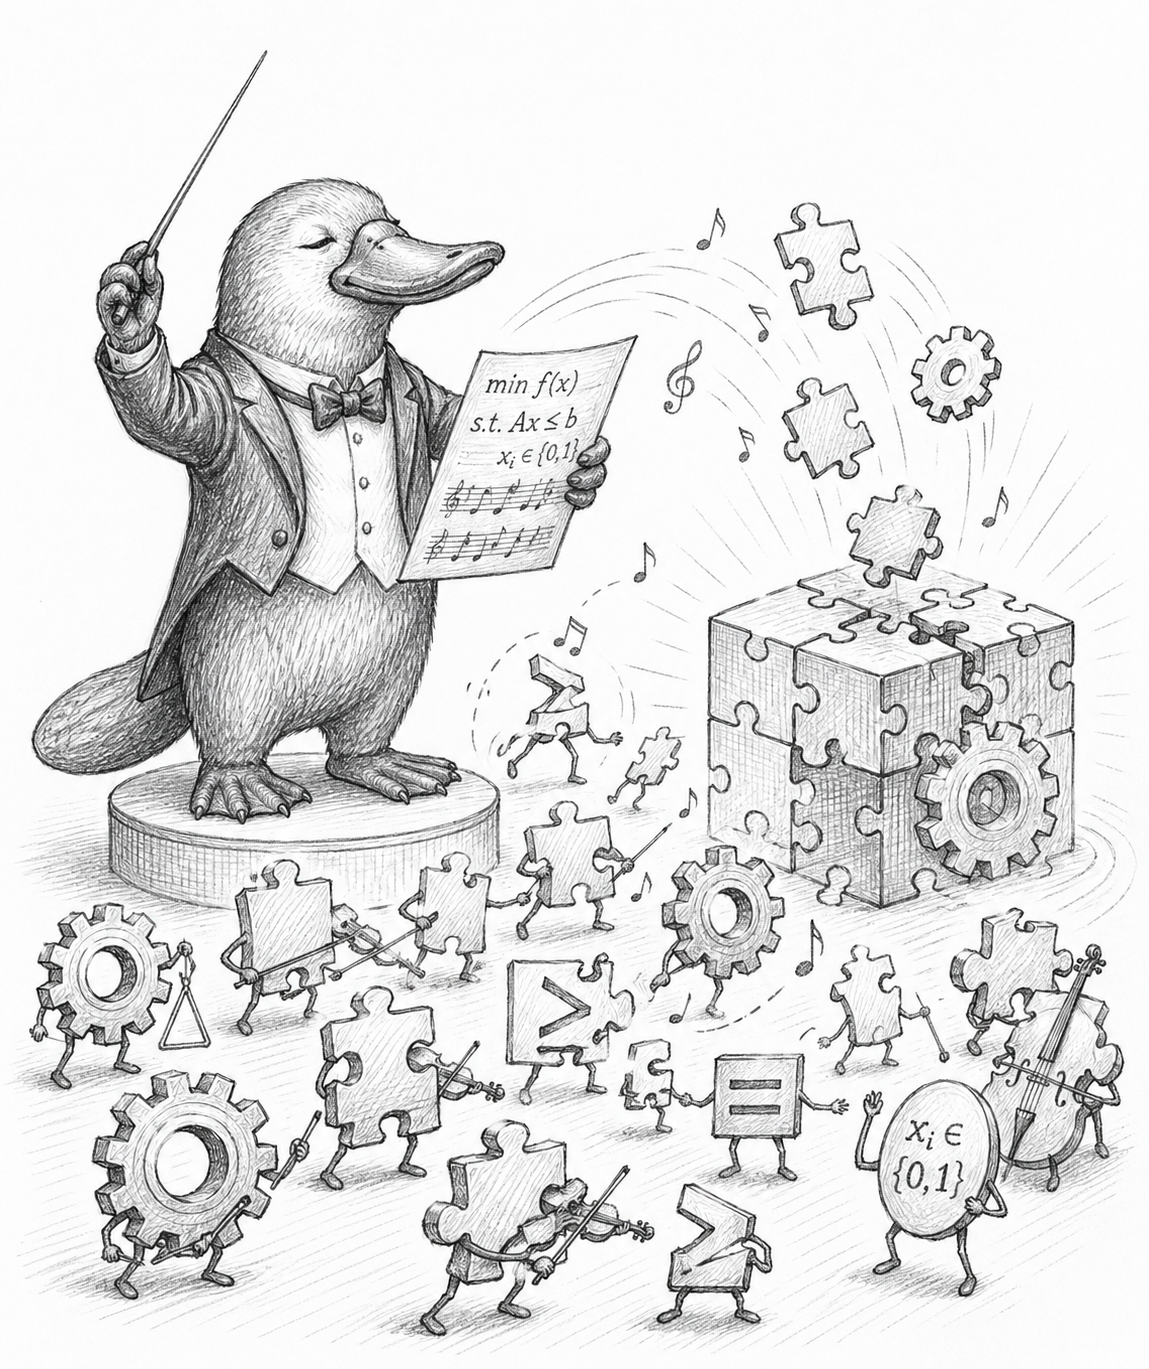
\includegraphics[width=0.55\textwidth]{cover.png}
    \vfill
    {\large Dominik Krupke\par}
    \vspace{0.3em}
    {\normalsize Algorithms Division, TU Braunschweig\par}
    \vspace{0.2em}
    {\small\href{mailto:krupked@gmail.com}{krupked@gmail.com}\par}
    \vspace{1.2em}
    {\footnotesize
      \raisebox{-0.35em}{\doclicenseImage[imagewidth=3em]}\quad
      \textcopyright\ Dominik Krupke. Licensed under
      \href{https://creativecommons.org/licenses/by/4.0/}{CC~BY~4.0}.\par}
    \vspace{0.4em}
    {\footnotesize\href{https://github.com/d-krupke/cpsat-primer}{github.com/d-krupke/cpsat-primer}\par}
  \end{titlepage}
}

% Path to platypus icon assets
\newcommand{\platypusassets}{.assets}

% ── Platypus callouts ────────────────────────────────────────────────
%
% Design: thick colored left rule, pale tinted background, no other
% borders. Platypus icon sits in the top-left margin; the title is set
% inline as the first paragraph of the body, in the accent color.
%
% Usage:
%   \begin{platypusinfo}     ... \end{platypusinfo}      % default title
%   \begin{platypusinfo}[Aside] ... \end{platypusinfo}   % custom title
%
% Variants: platypusinfo (blue), platypustip (green),
%           platypuswarning (amber), platypusbook (violet).

% Width allotted to the icon column (and reserved on the left of the body).
\newlength{\platypusiconwidth}
\setlength{\platypusiconwidth}{42pt}
\newlength{\platypusiconsep}
\setlength{\platypusiconsep}{12pt}

% Title style for the heading at the top of each box's body column.
\newcommand{\platypustitle}[2]{%
  {\bfseries\sffamily\large\color{#1!55!black}#2}\par\vspace{2pt}%
}

% Shared base. Argument 1 = accent color, 2 = icon basename, 3 = title text.
%
% Layout: the upper content is split into two top-aligned minipages —
% icon on the left, title+body on the right. Both columns participate in
% the box's natural height, so the frame always extends at least as far as
% the (potentially tall) platypus icon. Trade-off: minipage-based boxes
% cannot break across pages.
\tcbset{
  platypusbase/.style n args={3}{%
    enhanced,
    sharp corners,
    boxrule=0pt,
    leftrule=3pt,
    colback=#1!4,
    colframe=#1!55!black,
    left=12pt,
    right=12pt,
    top=12pt,
    bottom=12pt,
    fontupper=\normalsize,
    before upper={%
      \begin{minipage}[t]{\platypusiconwidth}%
        \vspace{0pt}% align minipage by its top, not first-line baseline
        \includegraphics[width=\platypusiconwidth,keepaspectratio]%
          {\platypusassets/platypus_#2}%
      \end{minipage}%
      \hspace{\platypusiconsep}%
      \begin{minipage}[t]{\dimexpr\linewidth-\platypusiconwidth-\platypusiconsep\relax}%
        \vspace{0pt}%
        \platypustitle{#1}{#3}%
    },
    after upper={\end{minipage}}%
  }
}

\newtcolorbox{platypusinfo}[1][Note]{%
  platypusbase={blue}{info}{#1}%
}

\newtcolorbox{platypustip}[1][Tip]{%
  platypusbase={green!60!black}{tip}{#1}%
}

\newtcolorbox{platypuswarning}[1][Warning]{%
  platypusbase={orange!85!black}{warning}{#1}%
}

\newtcolorbox{platypusbook}[1][Background]{%
  platypusbase={violet}{book}{#1}%
}


% --- Document metadata ----------------------------------------------------
\title{Declarative Modeling with CP-SAT}
\author{Dominik Krupke --- Algorithms Division, TU Braunschweig}
\date{}

\begin{document}

\maketitle

% --- Abstract -------------------------------------------------------------
\thispagestyle{empty}
\vspace*{2cm}
\begin{center}
{\Large\bfseries Abstract}
\end{center}
\vspace{0.8cm}
\noindent
When combinatorial problems grow beyond what ad hoc modeling can handle,
hands-on solver experience alone is not enough. Modelers need a structured way
to reason about the problem before writing solver code. This manuscript
presents such a structure, organized around four ideas: mathematical notation
is a working tool rather than a gatekeeping ritual; optimization models
decompose cleanly into five parts: entities, parameters, decision variables,
constraints, and an objective; a \emph{verifier}, implemented as a lightweight
Python function that judges the feasibility and quality of candidate solutions,
provides an orthogonal contract on what the problem actually means,
independent of any solver; and the choice of solver shapes how a model is best
expressed, with this manuscript committing to CP-SAT.

\vspace{0.6cm}
\noindent
This manuscript accompanies the
\href{https://github.com/d-krupke/cpsat-primer}{CP-SAT Primer}, the broader and
more extensive resource, which covers CP-SAT in depth, including much of the
modeling material treated here, alongside a great deal more. This text is
deliberately narrower: it concentrates on the discipline of \emph{modeling}
itself, the path from an informal problem to a formulation that is correct
before it is ever handed to the solver. It overlaps with the Primer on
purpose, so that it stands on its own as a self-contained read rather than
requiring the Primer first.

\vspace{0.6cm}
\noindent
The manuscript focuses on managing the mental complexity of turning an
informal problem into a structured model. It does not aim to cover
optimization theory or solver internals in depth, nor does it provide a
comprehensive CP-SAT reference. Instead, it emphasizes a disciplined modeling
workflow that produces a correct formulation: one that a verifier can check
and a solver can execute. Performance engineering, which tightens formulations,
exploits structure, and tunes solvers, is treated as a subsequent step.

\vspace{0.6cm}
\noindent
The primary audience is computer scientists and software engineers with
experience in Python and basic discrete mathematics who want a systematic
approach to modeling combinatorial optimization problems. Readers with a
background in mathematical optimization will find much of the material
familiar, although the verifier concept may still offer a useful perspective.
\newpage

% --- Table of contents ----------------------------------------------------
\tableofcontents
\clearpage

% --- Chapters -------------------------------------------------------------
\chapter{From Procedure to Description}\label{chap:1}

\begin{quote}
\emph{``Civilization advances by extending the number of important
operations which we can perform without thinking about them.''} ---
Alfred North Whitehead
\end{quote}

A software engineer's instinct on a combinatorial problem is to design
an algorithm: pick a strategy --- greedy, backtracking, branch-and-bound,
dynamic programming --- and commit to the search structure, the data
structures, the order of exploration, the pruning rules. The skill is
real and worth keeping. Many problems are best solved by writing the
procedure that solves them.

On most real combinatorial problems, however, a hand-rolled procedure is
far from the state of the art. Industrial solvers represent decades of
accumulated engineering --- clause learning, constraint propagation,
restart strategies, parallel workers, instance-tuned heuristics --- that
no individual programmer can reproduce in a project. The pragmatic move
on a hard combinatorial problem is therefore not to write a solver, but
to \emph{describe} the problem in a form that an existing solver can
consume, and let that solver search.

This is a paradigm shift, not a swap of one technique for another. The
two mindsets answer different questions:

\begin{itemize}
\item
  The \textbf{procedural} view answers \emph{how do I compute an
  answer?} It is the perspective of an algorithm designer. The output is
  a procedure that, when run, produces a solution.
\item
  The \textbf{declarative} view answers \emph{what counts as an answer?}
  It is the perspective of a problem describer. The output is a
  \emph{model} --- a precise, executable statement of which
  configurations are acceptable and which is best.
\end{itemize}

Both views are legitimate, and a working optimization practitioner moves
between them. Most readers of this manuscript will have stronger code
intuition than mathematical-notation intuition; that intuition does not
become useless under the new paradigm --- most of the work is still code
--- but it has to be redirected, since the code you write here
\emph{describes} rather than \emph{executes}.

The solver we will commit to in this manuscript is \textbf{CP-SAT}, the
constraint-programming solver that ships inside Google's
\href{https://developers.google.com/optimization}{OR-Tools}. The choice
is not innocent: different solvers reward different idioms, and a model
written for CP-SAT will not be byte-for-byte the model you would write
for a mixed-integer programming solver or a SAT solver. The underlying
paradigm shift, and most of the modeling vocabulary, transfers without
change. The solver-specific details are local to the last few chapters.

\section{A Concrete Contrast: 0/1 Knapsack}\label{sec:1.1}

The classical \textbf{0/1 knapsack} makes the shift concrete. Given a
set of items \(I\), each with a weight \(w_i\) and a value \(c_i\), and
a knapsack of capacity \(C\), choose a subset of items whose total
weight does not exceed \(C\) and whose total value is as large as
possible. The problem is a useful contrast because both an algorithmic
recipe and a declarative formulation are short enough to fit on one
page.

\subsection{The procedural answer}\label{sec:1.1.1}

The textbook procedural solution is a dynamic program. We define a
table \lstinline!dp[i][w]! whose entry is the best total value
achievable using the first \(i\) items and capacity at most \(w\), and
we fill the table by deciding, for each \((i, w)\), whether to take
item \(i\) or leave it.

\begin{lstlisting}[language=Python]
def knapsack(weights, values, C):
    n = len(weights)
    dp = [[0] * (C + 1) for _ in range(n + 1)]
    for i in range(1, n + 1):
        for w in range(C + 1):
            dp[i][w] = dp[i - 1][w]
            if weights[i - 1] <= w:
                take = dp[i - 1][w - weights[i - 1]] + values[i - 1]
                if take > dp[i][w]:
                    dp[i][w] = take
    return dp[n][C]
\end{lstlisting}

Several non-trivial decisions sit inside that function. We chose the
recursion (take versus leave), the table layout (items by capacity),
the fill order (forward in \(i\), forward in \(w\)), and the off-by-one
indexing between the table and the input arrays. None of these
decisions is part of the \emph{problem}; all of them are part of one
possible \emph{solution}.

The running time is proportional to \(\lvert I \rvert \cdot C\), which
is \emph{pseudo-polynomial}: linear in the numerical value of \(C\),
not in the bits needed to write \(C\) down. When \(C\) reaches the
millions the table no longer fits in memory, and the algorithm becomes
unusable even for trivially small \(\lvert I \rvert\). Other
algorithmic approaches exist, but they tend to be even more complex to
implement.

\subsection{The declarative answer}\label{sec:1.1.2}

The same problem written as mathematics is three lines:

\[
\begin{aligned}
\max \quad      & \sum_{i \in I} c_i\, x_i \\
\text{s.t.} \quad   & \sum_{i \in I} w_i\, x_i \;\le\; C \\
                    & x_i \in \{0, 1\} && \forall i \in I.
\end{aligned}
\]

Read aloud: maximize the total value over a choice of items, subject to
the total weight not exceeding the capacity, where each \(x_i\) is a
binary decision (take or leave). Three lines describe the entire problem
and commit to no algorithm at all. This is the form a paper or a
textbook would use, and \Cref{chap:2} develops the notation needed to
read it fluently.

The translation from this math into a working CP-SAT model is almost
line-for-line:

\begin{lstlisting}[language=Python]
from ortools.sat.python import cp_model

model = cp_model.CpModel()
x = [model.new_bool_var(f"x_{i}") for i in I]

model.add(sum(w[i] * x[i] for i in I) <= C)
model.maximize(sum(c[i] * x[i] for i in I))

solver = cp_model.CpSolver()
solver.solve(model)
\end{lstlisting}

One Boolean variable per item, one linear inequality for the capacity,
one linear objective, one call to the solver. There is no loop over the
capacity, no table, no decision about the order of exploration. CP-SAT
does all of that internally. The gain, for this example, is primarily
\emph{modeling style}: the code mirrors the mathematical statement
directly and is easy to extend. For knapsack specifically, specialized
algorithms remain very strong baselines, so the point of the example is
the declarative form, not a claim that CP-SAT is the canonical fastest
method for this problem family.

\subsection{Comparing the two}\label{sec:1.1.3}

The two formulations differ in three ways that matter.

The first is performance. The dynamic program's \(\lvert I \rvert
\cdot C\) running time is fine for moderate capacities and bad for
large ones, while
CP-SAT inherits decades of constraint-solver research --- clause
learning, propagation, restarts, parallel workers --- none of which we
had to write. This does not mean CP-SAT is automatically the best method
for knapsack; on narrow problem classes a tailored algorithm is often
the right baseline. The declarative model gives access to the solver's
machinery without requiring its implementation.

The second is reading effort. The procedural version mixes the problem
with its solution: to read it six months from now, you have to
reconstruct why the recursion is what it is, why the loops run in this
order, and what each index means. The declarative version reads as a
problem statement --- every line corresponds to a fact about the
problem, and the model is reviewable and explainable in roughly the same
form a colleague would expect on a whiteboard.

The third is extensibility, and it is the deepest of the three. Suppose
a new requirement appears: items A and B are mutually exclusive, or at
least three of items C, D, E must be taken. In the dynamic program the
recursion changes, the table changes, possibly the time complexity
changes, and we are back at the whiteboard. In the declarative model
each new requirement is one extra line --- \(x_A + x_B \le 1\) for the
mutual exclusion, \(x_C + x_D + x_E \ge 3\) for the cardinality --- and
the solver absorbs the addition without any change to how the search
proceeds. Real problems mutate; their constraints arrive in waves, first
the one in the textbook, then the regulatory rule, then the customer's
preference, then the operational quirk. A model that absorbs new
constraints by adding lines is incomparably easier to maintain than a
procedure that has to be redesigned each time.

\section{Modeling, Not Magic}\label{sec:1.2}

Handing a problem to a solver does not make it easy. NP-hard problems
remain NP-hard; the solver does not abolish complexity, it merely
searches more cleverly than you would have. What changes with
declarative modeling is not whether the problem is hard but how large an
\emph{instance} you can practically solve.

This last point is where the real skill of optimization modeling lives.
The same problem can be encoded in many mathematically equivalent ways,
and the encodings differ enormously in how well a solver handles them. A
naive encoding may time out at fifty variables; an idiomatic encoding
may solve in two seconds at five thousand. The two models are saying the
same thing about the same problem, but only one of them is saying it in
a way the solver can exploit.

A few patterns recur. Solvers are tuned for certain shapes of
constraint, so a formulation that reaches for the solver's native
vocabulary --- global constraints, indicator variables, well-known
reformulations --- usually beats one that reinvents the same logic from
arithmetic primitives. Encodings that rule out symmetric or equivalent
solutions, removing duplicates the solver would otherwise explore,
outperform encodings that leave that freedom in, even when both are
mathematically correct. None of this is visible from the problem
statement; choosing the representation is part of the modeler's job, and
two correct models for the same problem can differ in solving time by
orders of magnitude.

The remaining chapters cover the basics to get you rolling with building
and solving your first models. Performance engineering of models is a
topic for later.

\section{What This Manuscript Develops}\label{sec:1.3}

Four ideas run through the rest of the book, and each one is the subject
of one or more chapters.

The first is that \emph{mathematical notation is a tool, not
gatekeeping}. Optimization papers and textbooks state problems in
notation because notation is shorter and less ambiguous than prose ---
not because the community is exclusive. Reading and writing it is a
habit anyone working with optimization can pick up. \Cref{chap:2} is a fast
alignment layer for that notation: sets, variables, expressions,
predicates, and the bridges between the numeric and Boolean parts of the
language.

The second is that \emph{optimization models decompose into five parts}:
the entities the problem talks about, the parameters that describe a
particular instance, the decision variables, the constraints that
restrict their combinations, and the objective that ranks the feasible
ones. This decomposition is the structure every model in the manuscript
uses. \Cref{chap:3} walks through it in a from-scratch recipe.

The third is that \emph{a verifier is an orthogonal contract on what the
problem actually means}. A verifier is a small piece of plain Python
that takes a candidate solution and answers two questions: is it valid,
and how good is it? It does not produce solutions; it judges them.
Writing one is independent of which solver eventually does the search,
and it pins the problem definition down in code so later modeling
decisions cannot drift away from it. \Cref{chap:4} develops the verifier
pattern; later chapters treat it as optional but useful.

The fourth is that \emph{knowing the solver's language matters}. The
same problem can be modeled in many mathematically equivalent ways, and
an idiomatic encoding for one solver looks different from an idiomatic
encoding for another. This manuscript commits to \textbf{CP-SAT}, the
constraint-programming solver that ships inside Google's
\href{https://developers.google.com/optimization}{OR-Tools}. CP-SAT has
an expressive vocabulary --- global constraints for routing, scheduling,
packing, and combinatorial structure --- and \Cref{chap:5}--\Cref{chap:8} lay it out: a
first end-to-end model, then variables, constraints, and objectives in
reference form. \Cref{chap:9} closes the manuscript by reflecting on these
four ideas and naming a few practical moves that come up in real
modeling work.

\begin{platypusinfo}
This manuscript works directly with CP-SAT's Python API
rather than with an algebraic modeling language such as AMPL, GAMS,
Pyomo, MiniZinc, or CPMpy. Algebraic modeling languages add a layer of
abstraction above solver APIs and often allow the same model to target
multiple solvers. They are valuable tools, but they would obscure the
solver-specific idioms this manuscript wants to teach. CP-SAT's Python
API is already high-level enough for introductory modeling, while still
exposing the modeling choices that matter for performance.
\end{platypusinfo}

\chapter{The Language of Optimization Models}\label{chap:2}

\begin{quote}
\emph{``A good notation has a subtlety and suggestiveness which at times
makes it almost seem like a live teacher.''} --- Bertrand Russell
\end{quote}

This chapter introduces a common notation for discrete optimization. The
focus is on MIP- and CP-style notation that dominates much of the
modeling literature; much of the same vocabulary carries over to SAT
modeling, even though that community uses its own surface syntax. Other
communities and textbooks adopt variants---different letter conventions,
bracket styles, and shorthands for global constraints---and we do not
claim that the choices below are universal.

Fluency in this notation yields three benefits. First, it makes research
papers and textbooks readable, allowing you to extract ideas rather than
rederive them. Second, once a problem exceeds what fits in working
memory, it is faster to sketch a precise model on paper than to move
directly to code. Third, it provides a shared, unambiguous language for
personal notes, whiteboard discussions, and paper drafts.

Most of the material is standard, and the chapter also serves as a
reference. If you are unsure how much you already know, use the section
headings as a checklist.

\section{Notation in Action}\label{sec:2.1}

Recall the 0/1 knapsack: items \(I\) with weights \(w_i\) and values
\(c_i\), a knapsack of capacity \(C\), and a binary choice per item.
Compressed into a single line, the model reads

\[
\max_{x \in \{0,1\}^{|I|}} \;\Bigl\{\, \sum_{i \in I} c_i\, x_i \;\;\Big|\;\; \sum_{i \in I} w_i\, x_i \le C \,\Bigr\}.
\]

This line specifies, in order, \emph{what we choose} (a binary vector
\(x\), one component per item), \emph{what we optimize} (a weighted sum
of values), and \emph{what is allowed} (the weighted sum of weights
does not exceed \(C\)). Each symbol is functional, and a reader
familiar with the conventions can reconstruct the problem without
additional prose.

Now suppose the values are uncertain: a simulator provides \(|S|\)
scenarios, and we require a packing that performs well in the worst
case. The model changes minimally:

\[
\max_{x \in \{0,1\}^{|I|}} \; \min_{s \in S} \;\Bigl\{\, \sum_{i \in I} c^s_i\, x_i \;\;\Big|\;\; \sum_{i \in I} w_i\, x_i \le C \,\Bigr\}.
\]

The decision variables, parameters, and constraint remain unchanged;
only the objective acquires a \(\min_{s \in S}\), and the values carry a
scenario index. The formulation remains flexible: replacing
\(\min_{s \in S}\) with \(\sum_{s \in S} p_s\) yields an expected-value
objective under scenario probabilities \(p_s\); replacing it with a
quantile operator yields a value-at-risk objective. The remainder of the
model is unaffected. In contrast, a prose formulation would require
substantial rewriting for each variant.

Next, consider two knapsacks: the original with capacity \(C\), and a
second with capacity \(C'\) that only accepts light items,
\(I' = \{i \in I \mid w_i \le w'\}\). We must choose one knapsack and
pack it, while still maximizing the worst-case value. Rather than
inlining everything into a single expression, define the feasible
regions:

\[
\mathcal{F}_0 \;=\; \bigl\{\, x \in \{0,1\}^{|I|} \;\big|\; \textstyle\sum_{i \in I} w_i x_i \le C \,\bigr\},
\]

\[
\mathcal{F}_1 \;=\; \bigl\{\, x \in \{0,1\}^{|I|} \;\big|\; \textstyle\sum_{i \in I} w_i x_i \le C',\;\; x_i = 0 \;\;\forall i \in I \setminus I' \,\bigr\},
\]

and combine them using a set union:

\[
\max_{x \;\in\; \mathcal{F}_0 \,\cup\, \mathcal{F}_1} \; \min_{s \in S} \;\sum_{i \in I} c^s_i\, x_i.
\]

Each line serves a distinct purpose. The decomposition also exposes
structure: the feasible regions \(\mathcal{F}_0\) and \(\mathcal{F}_1\)
are independent of the scenarios, whereas the objective depends on them.
Thus, uncertainty affects \emph{what is optimized}, not \emph{what is
feasible}. Once defined, these regions can be reused---for example, to
state bounds, define relaxations, or compare variants---without
repeating their definitions.

The notation integrates naturally with prose: symbols appear inline
(\(I'\), \(\mathcal{F}_1\)), in displayed equations, and across
paragraphs without friction. The two registers remain consistent and
mutually reinforcing.

The remainder of this chapter develops the vocabulary underlying these
examples: sets and indices, parameters, graphs, variables and domains,
expressions, objectives, constraints, and logical connectives.

\section{Sets, Indices, and Parameters}\label{sec:2.2}

Consider a city planning problem: choose locations for ambulance
stations. Let \(C\) denote the set of neighborhoods to serve and \(F\)
the set of candidate sites. The goal is to open as few stations as
possible while ensuring that every neighborhood lies within a
five-minute drive of at least one open station. A drive-time function
\(d : C \times F \to \mathbb{R}_{\ge 0}\) returns the travel time in
minutes; for \(c \in C\) and \(f \in F\), \(d(c, f)\) is the time from
\(c\) to \(f\). For a fixed site \(f \in F\), the neighborhoods
reachable within five minutes form a subset of \(C\):

\[
N_f \;=\; \{\, c \in C \;\mid\; d(c, f) \le 5 \,\}.
\]

The braces with a vertical bar denote \emph{set-builder notation}: all
elements of \(C\) that satisfy the condition. The subscript \(f\)
indicates that this defines one set per candidate site---an indexed
family \(\{N_f\}_{f \in F}\).

\begin{platypustip}
Maintain a table of sets and parameters as a glossary. For
the ambulance problem:

\begin{symboltable}{lL}
Symbol & Meaning \\ \midrule
\(C\) & set of neighborhoods to serve \\
\(F\) & set of candidate sites \\
\(d : C \times F \to \mathbb{R}_{\ge 0}\) & drive-time function \\
\(N_f\) & neighborhoods reachable from site \(f\) within five minutes \\
\end{symboltable}


If multiple variable types appear, create an analogous table for
variables, including their domains.
\end{platypustip}

The decision is to select a subset \(F^\star \subseteq F\) of sites to
open. The coverage requirement is

\[
\bigcup_{f \in F^\star} N_f \;=\; C.
\]

Given \(F^\star\), the neighborhoods uniquely covered by an open site
\(f \in F^\star\) are

\[
N_f \;\setminus\; \bigcup_{g \in F^\star \setminus \{f\}} N_g.
\]

If this set is empty, site \(f\) is redundant. Another useful
observation: if \(N_g \subseteq N_f\) for some \(g \in F\), then \(g\)
is dominated and can be removed from \(F\) before solving, since any
coverage it provides is already achieved by \(f\).

The set operators used above, along with several standard ones:

\begin{symboltable}{lL}
\(a \in A\) & membership: \(a\) is an element of \(A\) \\
\(a \notin A\) & non-membership: \(a\) is not an element of \(A\) \\
\(A \cup B\) & union: elements in \(A\) or \(B\) (or both) \\
\(A \cap B\) & intersection: elements in both \\
\(A \setminus B\) & difference: elements in \(A\) but not in \(B\) \\
\(A \subseteq B\) & subset relation \\
\(A \times B\) & Cartesian product: ordered pairs \((a,b)\) \\
\(\lvert A \rvert\) & cardinality: number of elements \\
\(\emptyset\) & empty set \\
\(\{a \in A \mid P(a)\}\) & set-builder notation \\
\end{symboltable}

Cartesian products describe relations and graphs: for example, an arc
set \(E \subseteq V \times V\), a set of feasible (worker, job)
assignments, or the edge set of a conflict graph.

A few naming conventions recur. Sets typically use uppercase Latin
letters, with corresponding lowercase symbols for elements: \(i \in I\),
\(j \in J\), \(v \in V\). Certain letters carry conventional
meanings---\(V, E\) for vertices and edges, \(T\) for time periods,
\(K\) for constraint indices---but these are conventions, not
requirements. A symbol is defined by its declaration, not by its name.

Data can be written in two interchangeable forms. A parameter may appear
as a subscripted quantity, such as \(w_i\) or \(a_{ij}\), or as a
function, such as \(d(c, f)\). Formally, these are equivalent:
\((w_i)_{i \in I}\) and \(w : I \to \mathbb{R}\) define the same
mapping. Subscripts are compact for tabulated data; functional notation
reads more naturally when arguments span multiple index sets or when the
value is conceptually computed (e.g., a distance or cost query). The
notation \(d(c, f)\) reflects the latter interpretation.

\section{Graphs}\label{sec:2.3}

A graph is a common form of structured set: a pair \(G = (V, E)\), where
\(V\) is a finite set of vertices and \(E \subseteq V \times V\) is a
set of arcs. Vertices are typically denoted by \(v\) (or \(w\) when
needed), and \((v, w) \in E\) denotes an arc from \(v\) to \(w\), often
abbreviated as \(vw\). An \emph{undirected graph} uses unordered pairs:

\[
G = (V, E), \qquad \{v, w\} \in E.
\]

The choice between directed and undirected graphs depends on the
application---flows are directed, whereas relationships such as
friendships are not. The modeling choice can significantly affect the
resulting formulation.

For a directed graph, the \emph{out-neighborhood} and
\emph{in-neighborhood} of a vertex \(v\) are

\[
N^+(v) = \{\, w \in V \mid (v, w) \in E \,\}, \qquad N^-(v) = \{\, u \in V \mid (u, v) \in E \,\}.
\]

The notation follows the standard upstream/downstream interpretation
\(u \to v \to w\): \(u\) is a predecessor of \(v\), and \(w\) is a
successor. For an undirected graph, there is a single neighborhood,

\[
N(v) = \{\, w \in V \mid \{v, w\} \in E \,\}.
\]

A related convention reserves \(\delta^+(v)\) and \(\delta^-(v)\) for
the \emph{sets of arcs} leaving and entering \(v\),

\[
\delta^+(v) = \{\, (v, w) \in E \,\}, \qquad \delta^-(v) = \{\, (u, v) \in E \,\}.
\]

The distinction matters in flow formulations, where the natural sums are
over arcs rather than over neighboring vertices.

A \emph{subgraph} is a pair \((V', E')\) with \(V' \subseteq V\) and
\(E' \subseteq E\). It is \emph{induced} by \(V'\) if its edge set
consists exactly of those edges in \(G\) with both endpoints in \(V'\):

\[
E' = \{\, (v, w) \in E \mid v, w \in V' \,\}.
\]

The same definition applies to undirected graphs by interpreting
\((v, w)\) as \(\{v, w\}\). We write \(G[V']\) for the subgraph induced
by \(V'\). Induced subgraphs underlie structures such as cliques,
independent sets, and dense subgraphs. For example, a clique is a set
\(V' \subseteq V\) such that \(G[V']\) is complete.

As an example, consider constructing a worker's shift from a set of
tasks \(T\). Each task \(t \in T\) has a start time \(s_t\) and an end
time \(e_t \ge s_t\), and transitioning from \(t\) to \(t'\) requires
time \(\tau_{t,t'} \ge 0\). The feasible sequences of tasks can be
represented as a graph with

\[
V = T \cup \{v_{\text{start}}, v_{\text{end}}\}, \qquad
E \;=\; \bigl\{\, (t, t') \in T \times T \;\big|\; e_t + \tau_{t,t'} \le s_{t'} \,\bigr\}
\;\cup\; \bigl(\{v_{\text{start}}\} \times T\bigr)
\;\cup\; \bigl(T \times \{v_{\text{end}}\}\bigr).
\]

An arc \((t, t')\) indicates that \(t'\) can follow \(t\) in a feasible
schedule. The vertices \(v_{\text{start}}\) and \(v_{\text{end}}\)
represent the beginning and end of the shift. Since \(e_t \ge s_t\) and
\(\tau \ge 0\), all arcs move forward in time, so \(G\) is a
\emph{directed acyclic graph} (DAG).

A single worker's schedule corresponds to a path from
\(v_{\text{start}}\) to \(v_{\text{end}}\) in \(G\). If every task must
be assigned to exactly one worker and each worker performs one feasible
sequence, then minimizing the number of workers is the minimum
path-cover problem on this DAG, which reduces to bipartite matching.
With per-arc costs, the same structure yields a minimum-cost flow
formulation, typically after splitting each task vertex to enforce that
exactly one unit of flow uses it.

\begin{platypustip}
Modeling a problem as a graph provides access to a broad
range of graph algorithms, which can serve as subroutines or, in some
cases, solve the problem directly, as in this example.
\end{platypustip}

\section{Variables and Domains}\label{sec:2.4}

The decision variables \(x_i\) in the Knapsack problem lived in
\(\{0, 1\}^{|I|}\)---one bit per item, indicating whether the item is
selected. Consider the same model with a modified domain:

\[
\max \;\sum_{i \in I} c_i\, x_i
\quad\text{s.t.}\quad
\sum_{i \in I} w_i\, x_i \le C,
\qquad x_i \in [0, 1].
\]

The objective, constraint, and data are unchanged; only the domain
differs. This is the \emph{fractional knapsack} problem, where items can
be taken in any proportion between zero and one. It admits a greedy
solution in \(\mathcal{O}(|I| \log |I|)\) time by sorting items by value
density. In contrast, the original formulation with \(x_i \in \{0,1\}\)
is NP-hard. Changing the domain again to \(x_i \in \mathbb{N}_0\) yields
the \emph{unbounded knapsack} problem, where any non-negative number of
copies of each item may be selected.

Each \(x_i\) is a \emph{decision variable}---a quantity determined by
the solver---and its \emph{domain} specifies the admissible values.
Common domains include:

\begin{symboltable}{lL}
Domain & Typical use \\ \midrule
\(\mathbb{R}\) & continuous quantities (flows, prices, fractions) \\
\(\mathbb{Z}\) & integers (indices, offsets) \\
\(\mathbb{N}_0\) & non-negative integers (counts, quantities) \\
\(\{0,1\}\) & binary decisions \\
\(\{1,2,\dots,k\}\) & finite enumerations (machines, modes) \\
\(\{\text{red}, \text{green}\}\) & symbolic enumerations \\
\end{symboltable}


Bounds are a special case of domains: \(l_i \le x_i \le u_i\) is
equivalent to \(x_i \in [l_i, u_i]\), and \(x_i \ge 0\) to
\(x_i \in [0, \infty)\). When multiple variables share a domain, we
write \(x \in \mathbb{R}^n\), \(x \in \mathbb{Z}^n\), or
\(x \in \{0,1\}^n\).

Variable names follow informal conventions---\(x\) for primary
decisions, \(y\) for auxiliary variables, \(s\) for slack variables, and
\(z\) for objective values---but these conventions are not binding.

\section{Expressions}\label{sec:2.5}

Expressions are quantities formed from variables and parameters; once
the variables are fixed, an expression evaluates to a scalar. It is
useful to distinguish between linear and nonlinear expressions, because
the distinction has algorithmic consequences. Models composed entirely
of linear expressions---\emph{linear programs} and \emph{mixed-integer
linear programs}---are significantly better understood than their
nonlinear counterparts. In practice, nonlinear formulations are often
transformed into linear ones, either exactly or through approximation.

\subsection{Linear expressions}\label{sec:2.5.1}

A linear expression is a weighted sum of variables:

\[
\sum_{i \in I} c_i x_i.
\]

This form appears in many contexts: total value in knapsack, total
assignment cost, or total flow into a vertex. Nested sums extend the
structure over Cartesian products:

\[
\sum_{i \in I} \sum_{j \in J} a_{ij} x_{ij}
\;=\;
\sum_{(i,j) \in I \times J} a_{ij} x_{ij}.
\]

The right-hand form is convenient when the index set is a subset of
\(I \times J\), such as the edge set of a graph:

\[
\sum_{(i,j) \in E} x_{ij}.
\]

In vector notation, \(\sum_i c_i x_i\) is written as \(c^\top x\), and a
system of linear constraints as \(A x \le b\). The indexed and vector
forms represent the same object, differing only in presentation.

\subsection{Nonlinear expressions}\label{sec:2.5.2}

Any expression that is not a linear combination of variables is
\emph{nonlinear}. Three common patterns recur.

The first consists of variables passed through nonlinear functions, such
as products or transcendental functions:

\[
x_i^2, \quad x_i x_j, \quad \exp(x_i), \quad \log(x_i).
\]

The second pattern aggregates over an index set, analogous to \(\sum\)
in \Cref{sec:2.5.1}, but produces a nonlinear result:

\[
\max_{i \in I} g_i(x), \quad \min_{i \in I} g_i(x), \quad
\operatorname{median}_{i \in I} g_i(x), \quad
\operatorname{mode}_{i \in I} g_i(x), \quad
\operatorname{quantile}_{i \in I}^{\,q} g_i(x).
\]

The third pattern connects logical predicates to numeric expressions.
The \emph{Iverson bracket} maps a predicate \(P\) to a binary value:

\[
[P] \;=\; \begin{cases} 1 & \text{if } P \text{ is true}, \\ 0 & \text{otherwise.} \end{cases}
\]

For example, the number of variables taking a specific value is

\[
\sum_{i \in I} [\, x_i = v \,],
\]

and the condition ``at most \(k\) of the predicates \(P_1, \dots, P_n\)
hold'' can be written as \(\sum_{i=1}^{n} [P_i] \le k\).

\subsection{Declaring functions}\label{sec:2.5.3}

A function is declared by specifying its \emph{signature}:

\[
f : A \to B,
\]

which defines the function name \(f\), its domain \(A\), and its
codomain \(B\). Optionally, a definition follows:

\[
f(a) := \dots.
\]

The domain and codomain may be Cartesian products, as in
\(d : C \times F \to \mathbb{R}_{\ge 0}\). This notation covers
parameters (data expressed as functions rather than indexed symbols),
derived expressions (e.g., \(\mathrm{slack}(x) := C - \sum_i w_i x_i\)),
and predicates (with codomain \(\{0,1\}\) or
\(\{\text{true}, \text{false}\}\)).

\begin{platypusinfo}
An optimization problem can itself be viewed as a
function: parameters map to an optimal value. For the 0/1 knapsack,
\begin{align*}
\mathrm{knapsack} :\; & \mathbb{R}_{\ge 0}^{n} \times \mathbb{R}_{\ge 0}^{n} \times \mathbb{R}_{\ge 0} \to \mathbb{R}_{\ge 0}, \\
\mathrm{knapsack}(c, w, C) \;=\; & \max_{x \in \{0,1\}^{n}} \Bigl\{\, \textstyle\sum_{i} c_i x_i \;\Big|\; \sum_i w_i x_i \le C \,\Bigr\}.
\end{align*}
\end{platypusinfo}

\section{Objectives}\label{sec:2.6}

An optimization problem selects \(x\) from a feasible region
\(\mathcal{F}\) to minimize a scalar objective \(f : D \to \mathbb{R}\):

\[
\min_{x \in \mathcal{F}} f(x).
\]

Maximization replaces \(\min\) with \(\max\), or equivalently
minimizes \(-f\). The minimum attained is the \emph{optimal value},

\[
f^\star = \min_{x \in \mathcal{F}} f(x),
\]

and the set of \emph{optimal solutions} is

\[
\arg\min_{x \in \mathcal{F}} f(x) \;=\; \{\, x \in \mathcal{F} \mid f(x) = f^\star \,\}.
\]

We write \(x^\star \in \arg\min\) rather than \(x^\star = \arg\min\),
because the optimum need not be unique; many problems admit multiple
optimal solutions, sometimes forming a continuum.

When multiple criteria are considered, we obtain a vector of objective
values \((f_1(x), \dots, f_m(x))\). Such vectors are not minimized by
the usual scalar order; one must choose a notion of preference, such as
Pareto dominance, a weighted sum, a minimax objective, or a
lexicographic order. The choice is a modeling decision and is not
pursued here.

\section{Constraints}\label{sec:2.7}

A constraint is a \emph{predicate}---a statement that evaluates to true
or false for a given assignment of values. While expressions answer
``what is the value?'', constraints answer ``is the condition
satisfied?''.

The most common predicates in optimization are linear (in)equalities:

\[
\sum_{j \in J} a_{ij} x_j \;\le\; b_i \qquad \forall i \in I.
\]

The quantifier \(\forall i \in I\) is essential: this defines a family
of \(|I|\) constraints, not a single one. For example, if
\(I = \{1,2,3\}\), the family expands to

\[
\sum_j a_{1j} x_j \le b_1, \qquad \sum_j a_{2j} x_j \le b_2, \qquad \sum_j a_{3j} x_j \le b_3.
\]

Equalities and reverse inequalities follow the same pattern.

Linearity is convenient but not required. In general, a constraint has
the form

\[
P_k(x) \qquad \forall k \in K,
\]

where each \(P_k\) is a predicate on the variable vector---for example,
a linear inequality, an \emph{AllDifferent} constraint, a
\emph{NoOverlap} constraint, or another relation.

\section{Logic and Quantifiers}\label{sec:2.8}

Many decisions are yes/no decisions: \emph{open this station},
\emph{take this course}, \emph{make this assignment}. A 0/1 variable is
enough to encode them. Models built from such Boolean variables use the
standard logical connectives

\[
\land, \quad \lor, \quad \neg, \quad \Rightarrow, \quad \Leftrightarrow,
\]

possibly quantified over index sets with \(\forall\) and \(\exists\).
Two common large-operator forms are

\[
\bigwedge_{k \in K} \phi_k, \qquad \bigvee_{k \in K} \phi_k.
\]

They denote the conjunction and disjunction of an indexed family of
Boolean expressions \(\phi_k\). The first is equivalent to the
constraint family \(\phi_k ;\forall k \in K\); the second means that at
least one \(\phi_k\) must hold, and therefore cannot be replaced by a
family of separate constraints.

\begin{center}\rule{0.5\linewidth}{0.5pt}\end{center}

\paragraph{Example.} After an office prank, three suspects remain: Anna,
Ben, and Cara. Let \(x_a, x_b, x_c \in \{0,1\}\) encode whether each
person is guilty. Witnesses provide four facts. Anna would only act with
Ben, so \(x_a \Rightarrow x_b\). Ben and Cara have never gotten along,
so \(\neg(x_b \land x_c)\). Cara would only join if Anna did, so
\(x_c \Rightarrow x_a\). Finally, someone did it, so
\(x_a \lor x_b \lor x_c\). Together, the facts give

\[
(x_a \Rightarrow x_b) \;\land\; \neg(x_b \land x_c) \;\land\; (x_c \Rightarrow x_a) \;\land\; (x_a \lor x_b \lor x_c).
\]

Chaining the implications gives \(x_c \Rightarrow x_a \Rightarrow x_b\).
But \(x_b\) implies \(\neg x_c\), because Ben and Cara cannot both be
guilty. Hence \(x_c \Rightarrow \neg x_c\), so \(x_c = 0\). With Cara
cleared, the condition that someone is guilty reduces to
\(x_a \lor x_b\). Together with \(x_a \Rightarrow x_b\), this forces
\(x_b = 1\), regardless of Anna's role. The clues implicate Ben, clear
Cara, and leave Anna's status undetermined.

\begin{center}\rule{0.5\linewidth}{0.5pt}\end{center}

The connectives are not limited to Boolean variables; they also compose
predicates over richer variables. Suppose two jobs share a machine. With
start times \(s_1, s_2 \in \mathbb{N}_0\) and durations \(d_1, d_2\),
the jobs must run one after the other:

\[
s_1 + d_1 \le s_2 \;\;\lor\;\; s_2 + d_2 \le s_1.
\]

This is a disjunction of two linear inequalities over integer variables.
The same logical connectives apply to inequalities, equalities,
\(\text{AllDifferent}(y_1,\ldots,y_k)\), \(\text{NoOverlap}\)
constraints, or any other relation. A predicate, like a function, can be
named for reuse:

\[
P(x) \;:=\; \sum_{i \in I} w_i x_i \le C.
\]

Once named, it fits into the same logical syntax:
\(P_1(x) \land P_2(x)\), \(P(x) \Rightarrow Q(x)\), or
\(\bigvee_{k \in K} P_k(x)\).

The two layers---Boolean variables and predicates over richer
variables---meet in \emph{reification}. Reification ties a Boolean
indicator \(z \in \{0,1\}\) to the truth value of a predicate:

\[
z \;\Leftrightarrow\; (x \ge 5).
\]

Once reified, \(z\) can appear in logical connectives like any other
Boolean variable. The special case \(z \Rightarrow a^\top x \le b\) is
known as an \emph{indicator constraint} in MIP terminology. How a solver
encodes such patterns is separate from how the model states them.

\section{A Standard Model Template}\label{sec:2.9}

Many optimization models share a common skeleton. In its simplest form,
it is

\[
\begin{aligned}
\min_{x} \quad      & f(x) \\
\text{s.t.} \quad   & P_k(x) && \forall k \in K, \\
                    & x \in D.
\end{aligned}
\]

The objective \(f\), predicates \(P_k\), and domain \(D\) are specified
by the application. The corresponding feasible region is

\[
\mathcal{F} = \{\, x \in D \mid P_k(x) \;\forall k \in K \,\},
\]

with optimal value and optimal solution written as

\[
f^\star = \min_{x \in \mathcal{F}} f(x),\qquad
x^\star \in \arg\min_{x \in \mathcal{F}} f(x).
\]

Many formulations you encounter will fit this template, often with only
minor notational variations.

\chapter{Drafting the Model}\label{chap:3}

\begin{quote}
\emph{``All models are wrong, but some are useful.''} --- George E. P.
Box
\end{quote}

There are two fundamental challenges to overcome before implementing an
optimization model in a solver. The first is to express the problem in a
precise form. The second is to translate that form into something the
interface of your chosen solver can understand. Further challenges will
follow later, especially making the model run fast, but this chapter
focuses only on the first two.

The previous chapter gave us the notation needed to start sketching a
model. In this chapter, we look at a structured way to do so. The
structure is not linear: for a complicated problem, you usually identify
the core, formulate it, get it into a runnable form, and then extend it
with the remaining rules and objectives.

The five modeling ingredients in this chapter --- entities, parameters,
variables, constraints, and objective --- are therefore not a checklist
that you complete once. They are a recurring guide. New constraints may
require new variables; a new objective term may change which parameters
matter; a newly discovered entity may force you to restructure earlier
parts of the formulation. With experience, the iterations tend to become
fewer and smaller.

\section{The Five Components}\label{sec:3.1}

A complete optimization model has five components that provide structure
for thinking and writing:

\begin{enumerate}
\item
  \textbf{Entities} --- what objects does the problem talk about? They
  become \emph{sets}.
\item
  \textbf{Parameters} --- what data is known up front? They become
  \emph{constants indexed by the sets}.
\item
  \textbf{Variables} --- what is the solver allowed to choose? They
  become \emph{unknowns with a domain}.
\item
  \textbf{Constraints} --- what makes a choice valid? They become
  \emph{relations on variables}.
\item
  \textbf{Objective} --- what makes one valid choice better than
  another? It becomes \emph{one expression with sense
  \lstinline!min! or \lstinline!max!};
  multi-objective optimization is a topic of its own.
\end{enumerate}

The order is a guideline. Entities and parameters define the language;
variables depend on that language; constraints relate the variables; the
objective evaluates valid choices.

For the Knapsack problem from the previous chapter, the five components
read:

\begin{enumerate}
\item
  \textbf{Entities.} The items, \(I\).
\item
  \textbf{Parameters.} A value \(c_i \in \mathbb{R}_{\ge 0}\) and a
  weight \(w_i \in \mathbb{R}_{\ge 0}\) for every \(i \in I\), plus a
  knapsack capacity \(C \in \mathbb{R}_{\ge 0}\).
\item
  \textbf{Variables.} One binary variable per item, \(x_i \in \{0, 1\}\)
  for \(i \in I\), with \(x_i = 1\) meaning \emph{take item \(i\)}.
\item
  \textbf{Constraints.} The total weight must not exceed capacity:
  \(\sum_{i \in I} w_i x_i \le C\).
\item
  \textbf{Objective.} Maximize total value:
  \(\max \sum_{i \in I} c_i x_i\).
\end{enumerate}

Now suppose we want to integrate the scenario-based worst-case objective
from the previous chapter. We have to change a few components, but the
model still looks similar:

\begin{enumerate}
\item
  \textbf{Entities.} Items \(I\) and scenarios \(S\).
\item
  \textbf{Parameters.} A per-scenario value
  \(c_i^s \in \mathbb{R}_{\ge 0}\) for every \(i \in I\) and
  \(s \in S\); weights \(w_i\) and capacity \(C\) as before.
\item
  \textbf{Variables.} Unchanged: \(x_i \in \{0, 1\}\) for \(i \in I\).
\item
  \textbf{Constraints.} Unchanged: \(\sum_{i \in I} w_i x_i \le C\).
\item
  \textbf{Objective.} Maximize the worst-case value:
  \(\max \min_{s \in S} \sum_{i \in I} c_i^s x_i\).
\end{enumerate}

This is a precise paper formulation, but it is not yet in a form
suitable for most solvers. The objective contains a \(\min\) over
scenarios inside the maximization, and most solvers will not accept that
nested expression as written. The standard remedy is an
auxiliary-variable reformulation: introduce a variable \(z\) for the
worst-case value and bound it from above by every scenario's value.

The solver-facing version is:

\begin{enumerate}
\item
  \textbf{Entities.} Items \(I\) and scenarios \(S\).
\item
  \textbf{Parameters.} \(c_i^s\), \(w_i\), and \(C\).
\item
  \textbf{Variables.} \(x_i \in \{0, 1\}\) for \(i \in I\), and an
  auxiliary variable \(z\) representing the worst-case value.
\item
  \textbf{Constraints.} The capacity constraint \[
  \sum_{i \in I} w_i x_i \le C,
  \] and the scenario-value constraints \[
  z \le \sum_{i \in I} c_i^s x_i \qquad \forall s \in S.
  \]
\item
  \textbf{Objective.} Maximize \(z\).
\end{enumerate}

Maximizing \(z\) subject to one inequality per scenario forces \(z\) up
to the smallest scenario value, recovering the original
\(\min_{s \in S}\) exactly.

\section{A Worked Example: Hospital Ward Rostering}\label{sec:3.2}

Consider the following problem. A small hospital ward needs to schedule
its nursing staff for the coming week. The ward has a fixed list of
shifts to fill. Each shift has a date, a required skill --- say,
\emph{ICU}, \emph{pediatrics}, or \emph{general care} --- and a
headcount specifying how many nurses must be on duty. The ward employs a
roster of nurses, each of whom holds a personal set of skills and is
available on certain days but not others. Assigning a particular nurse
to a particular shift incurs a cost that captures wage rates, shift
differentials, and union overtime rules.

The ward manager wants to staff every shift, respect availability and
skills, and spend as little as possible.

We will now extract the five components. Unlike in the knapsack example,
they are no longer almost forced by the problem statement. We have
several kinds of objects, several indexed data tables, and constraints
that refer to different combinations of workers, shifts, days, and
skills. The point of the five-component structure is to keep that
complexity visible and organized.

\subsection{Step 1 --- Entities become sets}\label{step-1-entities-become-sets}

Read the problem statement and underline every noun that names a class
of objects. \emph{Nurses, shifts, days, skills.} Each class becomes a
set.

\begin{symboltable}{lL}
Symbol & Description \\ \midrule
\(W\) & Workers (nurses) --- the staff to be scheduled. \\
\(S\) & Shifts --- the work blocks to be filled this week. \\
\(T\) & Days --- the calendar dimension, \(T = \{1, \dots, 7\}\). \\
\(K\) & Skills --- the qualifications the ward tracks. \\
\end{symboltable}


A set is the \emph{type} of an index. Once we have written \(w \in W\)
and \(s \in S\), we can index any quantity in the model by \((w, s)\)
--- variables, parameters, constraints, neighborhoods.

\subsection{Step 2 --- Parameters are the input data}\label{step-2-parameters-are-the-input-data}

Anything known before we solve is a parameter. Parameters are often
indexed by the sets from step 1, and each one should carry a domain ---
the values it may take --- together with an informal description that
fixes what the symbol means. Some parameters are raw input data; others
are derived from that input to make the model easier to write.

\begin{symboltable}{lllL}
Symbol & Indices & Domain & Description \\ \midrule
\(c_{w,s}\) & \(w \in W,\; s \in S\) & \(\mathbb{R}_{\ge 0}\) & Cost of assigning worker \(w\) to shift \(s\). \\
\(a_{w,s}\) & \(w \in W,\; s \in S\) & \(\{0, 1\}\) & Availability flag: \lstinline!1! iff \(w\) is available for \(s\). \\
\(r_s\) & \(s \in S\) & \(K\) & Skill required by shift \(s\). \\
\(h_w\) & \(w \in W\) & \(2^K\) & Set of skills held by worker \(w\). \\
\(n_s\) & \(s \in S\) & \(\mathbb{N}_0\) & Number of workers needed on shift \(s\). \\
\(S_t\) & \(t \in T\) & \(2^S\) & Subset of shifts that fall on day \(t\) (derived from shift dates). \\
\end{symboltable}


The domains are explicit. \(c_{w,s}\) is a non-negative real,
\(a_{w,s}\) is binary, \(n_s\) is a non-negative integer, and \(h_w\) is
a subset of \(K\) (so its domain is the power set \(2^K\)). Each shift
requires one skill, while each worker may hold multiple skills --- a
detail that matters once we write the skill-match constraint.

The last row illustrates that a parameter need not be raw input. \(S_t\)
is derived from the dates of the shifts: for each day \(t\), it collects
exactly those shifts that occur on that day. Including such derived
parameters in the table is useful because it gives later constraints a
clean vocabulary. Instead of repeatedly writing ``all shifts that fall
on day \(t\),'' we can simply write \(S_t\).

\subsection{Step 3 --- Variables are the unknowns}\label{step-3-variables-are-the-unknowns}

This is the step where the problem stops being only a description and
becomes a model. Each decision unit becomes one variable, declared with
three things: a name, an index range, and a domain. What counts as a
single decision unit is itself a modeling choice: the same problem can
often be modeled at different granularities, with real consequences for
solver performance.

For the rostering problem, the natural first decision unit is \emph{does
worker \(w\) take shift \(s\)?} --- one binary choice per worker--shift
pair.

\begin{symboltable}{lllL}
Symbol & Indices & Domain & Description \\ \midrule
\(x_{w,s}\) & \(w \in W,\; s \in S\) & \(\{0, 1\}\) & \lstinline!1! iff worker \(w\) is assigned to shift \(s\), else \lstinline!0!. \\
\end{symboltable}


That single line declares \(|W| \cdot |S|\) variables --- one per cell
of the worker--shift matrix. Many of those combinations may be trivially
infeasible: the worker may be unavailable, or may lack the skill
required by the shift. In the simple formulation, we still declare the
full matrix and let constraints rule out the invalid combinations.

One could prune the index set up front and create variables only for
worker--shift pairs that are possible in principle. That is often a
useful implementation choice, but it is not needed for the first paper
model. At this stage, the full matrix is easier to read: every potential
assignment has a variable, and every rule appears explicitly as a
constraint. If an implementation detail is important enough to remember,
record it as a note rather than complicating the first formulation.

The decision here is \emph{take or leave}, so the natural variable is
binary. Other problems suggest other shapes:

\begin{symboltable}{lL}
Decision phrasing & Variable shape \\ \midrule
``Take it or not?'' & \(x_i \in \{0, 1\}\) --- binary \\
``How many?'' & \(x_i \in \mathbb{N}_0\) --- non-negative integer \\
``When does it start?'' & \(\text{st}_i \in [0, H]\) --- time variable, bounded by horizon \(H\) \\
``Which slot does it go into?'' & either \(x_i \in \{1, \dots, K\}\) \emph{or} \(y_{i,k} \in \{0,1\}\) --- index \emph{vs.} one-hot \\
``Which edge is used?'' & \(x_{ij} \in \{0,1\} \;\forall (i,j) \in E\) --- one Boolean per edge \\
\end{symboltable}


The fourth row deserves attention because it is a common modeling
decision: when the answer is ``which of \(K\) options,'' do you use a
single integer variable taking values in \(\{1, \dots, K\}\), or \(K\)
Boolean variables that sum to 1? Both can be correct. They differ in the
kinds of constraints they make easy to write and in the structure a
solver can exploit.

\begin{platypusinfo}
Real workforce-scheduling systems often use more
aggregate variables than the simple worker--shift assignment variable
above. In a column-generation model, for example, a variable may
represent an entire shift pattern for one worker over the planning
horizon. Since the number of possible patterns is usually enormous, the
model is solved iteratively: start with a manageable subset of patterns,
solve the restricted model, then generate additional useful patterns
through a separate pricing problem. That is a powerful technique, but it
is a different modeling level from the first paper formulation developed
here.
\end{platypusinfo}

\subsection{Step 4 --- Constraints encode validity}\label{step-4-constraints-encode-validity}

Constraints are usually the most complex part of the model. For simple
textbook examples, it may be enough to translate each ``must'' sentence
directly into one formula. But even the scenario-based knapsack example
showed that this is not always the whole story: sometimes a clear paper
statement needs auxiliary variables and additional constraints before it
becomes solver-friendly. In richer applications, one must also
distinguish between hard constraints, which define feasibility, and soft
constraints, which may be violated at a penalty. The present example is
cleanly specified, so we can ignore soft constraints for now.

We now identify the constraint families and formulate them one by one.
For hard constraints, each new rule narrows the feasible region: it
removes assignments that are not allowed, but it does not make
previously invalid assignments valid. This makes constraints relatively
modular. Still, a single rule may require several formulas, and part of
a rule may already be enforced by earlier constraints or by variable
domains. In this example, however, the mapping is pleasantly direct:
four business rules become four constraint families.

\paragraph{Coverage.} Every shift must be staffed with exactly the
headcount it requires.

\[
\sum_{w \in W} x_{w,s} \;=\; n_s \qquad \forall s \in S.
\]

This is one equation per shift. The sum on the left counts the number of
workers assigned to \(s\), and the right-hand side is the demanded
headcount. The \(\forall s \in S\) is doing real work: it makes this not
a single equation but a family of \(|S|\) equations.

\paragraph{Availability.} A worker may not be assigned to a shift they are
not available for.

\[
x_{w,s} \;\le\; a_{w,s} \qquad \forall w \in W, \; s \in S.
\]

If \(a_{w,s} = 0\), the inequality forces \(x_{w,s} = 0\). If
\(a_{w,s} = 1\), the inequality becomes \(x_{w,s} \le 1\), which is
already implied by the variable's domain, so the constraint is silent.

\paragraph{Skill match.} If a worker is assigned to a shift, the worker
must hold the skill the shift requires.

\[
x_{w,s} = 1 \;\Rightarrow\; r_s \in h_w \qquad \forall w \in W, \; s \in S.
\]

This is a clear paper-level statement, but it is not the most useful
solver-facing form because the right-hand side is a fact about the input
data, not a decision. The direct rewrite is:

\[
x_{w,s} \;\le\; [r_s \in h_w] \qquad \forall w \in W, \; s \in S,
\]

where the indicator on the right is \lstinline!1! if the
skill requirement is met and \lstinline!0! otherwise. The
compatibility values are computed from the data before the solver is
called; incompatible pairs are forced to zero, compatible pairs are left
to the other constraints.

\paragraph{No double-booking.} No worker may be assigned to more than one
shift on the same day.

\[
\sum_{s \in S_t} x_{w,s} \;\le\; 1 \qquad \forall w \in W, \; t \in T.
\]

For every worker--day combination, the sum runs only over the shifts
that fall on that day and requires that no more than one of them be
assigned to this worker. This is a typical use of a derived parameter
(\(S_t\)) to keep the constraint readable.

\subsection{Step 5 --- The objective picks among valid choices}\label{step-5-the-objective-picks-among-valid-choices}

We have specified what counts as a valid roster. Now we say which valid
roster we prefer.

\paragraph{Total cost.} Minimize the total cost of the assignments we make.

\[
\min \;\sum_{w \in W} \sum_{s \in S} c_{w,s} \, x_{w,s}.
\]

The sum runs over all worker--shift pairs, but only the pairs with
\(x_{w,s} = 1\) contribute.

Two notes on objectives. First, the sense ---
\lstinline!min! or \lstinline!max! --- is
part of the specification; ``optimize \(f\)'' is incomplete. Second, an
objective is a single expression. If the problem talks about several
goals at once --- cost \emph{and} overtime \emph{and} fairness --- you
must combine them yourself, by weighted sum or lexicographic ordering.
There is no implicit averaging. And a model can have no objective at
all: pure feasibility (``is \emph{any} valid roster possible?'') is a
legitimate question, and forcing an artificial objective onto it is a
mistake.

\chapter{Verifying Candidate Solutions}\label{chap:4}

\begin{quote}
\emph{``Show me your flowchart and conceal your tables, and I shall
continue to be mystified. Show me your tables, and I won't usually need
your flowchart; it'll be obvious.''} --- Fred Brooks, \emph{The Mythical
Man-Month}
\end{quote}

In this chapter, we discuss a concept that is orthogonal to the basic
modeling process. A \emph{verifier} is a piece of code that takes an
instance and a candidate solution, checks whether the solution is
feasible, and computes its objective value.

Writing such a verifier still requires the same five ingredients from
optimization modeling: entities, parameters, variables, constraints, and
objective. In the verifier, however, the variables appear as concrete
values inside a candidate \lstinline!Solution!, not as
symbolic objects controlled by a solver. The difference is the medium.
Instead of expressing the problem as mathematical notation or as solver
constraints, we express it as ordinary program code. For many software
engineers, this feels less abstract and more natural.

A verifier can be developed independently of the solver model, but the
two must agree on the problem definition and on the representation of
instances and solutions. Once available, the verifier can serve several
roles. It can help you test hand-written examples, evaluate simple
heuristics, and get a feel for the problem before the solver model is
mature. During solver development, it acts as a guardrail:
solver-produced solutions can be checked against it, random instances
can be smoke-tested, and performance-driven refactors can be validated
against the same problem definition.

In that sense, the verifier can be viewed as an executable contract for
the problem definition. It does not say how to find a good solution. It
says how to recognize a valid one, and how to score it once found.

\section{What a Verifier Is}\label{sec:4.1}

A verifier checks candidate solutions. Given an instance and a proposed
solution, it answers two questions:

\begin{enumerate}
\item
  Is the solution feasible?
\item
  What is its objective value?
\end{enumerate}

It does not search for solutions. It does not call a solver. It is not
an algebraic modeling language and not a solver model. A solver model
describes a search space to an optimization engine; a verifier checks
one fully specified candidate after the decisions have already been
made. Solvers produce solutions; verifiers consume them.

This difference makes a verifier much easier to write for many rules. In
a solver model, a rule must be expressed as a constraint over decision
variables, in the vocabulary supported by the solver. In a verifier, the
candidate assignment is already known, so the rule can be checked with
ordinary program code: branches, lookups, loops, early returns, and
descriptive error messages.

The \textbf{simple form} keeps all checks in one evaluator function. It
returns the objective value if the candidate is feasible and raises an
exception naming the first violated rule otherwise. This is short,
readable, and sufficient for many small hard-constraint models.

The \textbf{richer form} decomposes the checks into separate rule
modules and replaces yes/no answers with quantitative metrics:
\emph{three minutes of overlap}, \emph{two uncovered shifts}, \emph{one
missing skill}. This becomes useful once rules are soft, violations need
to be reported in bulk, or several solution methods need to be compared
against the same standard.

\section{\texorpdfstring{The Simple Form: \texttt{Instance}, \texttt{Solution}, \texttt{evaluate}}{The Simple Form: Instance, Solution, evaluate}}\label{sec:4.2}

A simple verifier consists of three pieces. The first two are plain data
containers and can be reused elsewhere in the codebase:

\begin{enumerate}
\item
  \textbf{\lstinline!Instance!}, a frozen dataclass
  holding the input data.
\item
  \textbf{\lstinline!Solution!}, a frozen dataclass
  holding one completed candidate solution.
\item
  \textbf{\lstinline!evaluate(instance, solution)!}, a
  pure function that checks feasibility and, if the solution is
  feasible, returns its objective value. If a constraint family fails,
  it raises an exception that identifies the failing rule.
\end{enumerate}

This is the minimal pattern: two dataclasses and one function. We illustrate it with a rostering verifier.

\subsection{Type Aliases for the Index Sets}\label{sec:4.2.1}

Python is dynamically typed, but type annotations are useful as
documentation and for static analysis and editor support. Here, we use
simple aliases for the index sets from the paper model:

\begin{lstlisting}[language=Python]
type Worker = str  # Identifier for a worker who can take shifts
type Shift  = str  # Identifier for a shift that needs to be staffed
type Day    = int  # Integer day index, e.g., 0 for Monday, 1 for Tuesday
type Skill  = str  # Skill that workers may hold and shifts may require
\end{lstlisting}

Workers, shifts, days, and skills are still strings or integers at
runtime. The aliases do not add type safety by themselves, but they
improve the shape of the code:
\lstinline!dict[tuple[Worker, Shift], int]! says more than
\lstinline!dict[tuple[str, str], int]!.

\subsection{\texorpdfstring{The \texttt{Instance} and \texttt{Solution} dataclasses}{The Instance and Solution dataclasses}}\label{sec:4.2.2}

\begin{lstlisting}[language=Python]
from dataclasses import dataclass

@dataclass(frozen=True)
class Instance:
    workers: frozenset[Worker]
    shifts:  frozenset[Shift]
    days:    frozenset[Day]
    skills:  frozenset[Skill]

    cost:           dict[tuple[Worker, Shift], int]
    available:      dict[tuple[Worker, Shift], bool]
    required_skill: dict[Shift,  Skill]
    holds_skills:   dict[Worker, frozenset[Skill]]
    headcount:      dict[Shift,  int]
    shifts_on_day:  dict[Day,    frozenset[Shift]]

@dataclass(frozen=True)
class Solution:
    assigned: frozenset[tuple[Worker, Shift]]
\end{lstlisting}

The \lstinline!Instance! carries the sets and parameters
from the math model; the \lstinline!Solution! carries the
values of the decision variables. The solution uses the \emph{sparse}
representation (we record only the pairs where \(x_{w,s} = 1\), not
the full zero-one matrix) which scales with what was assigned rather
than with the size of the index space.

\begin{platypusinfo}
For teaching purposes we use
\lstinline!dataclass!, but at the system boundary,
wherever an instance is built from a CSV, a database, or a JSON payload,
a properly validated data schema (typically
\href{https://docs.pydantic.dev/}{Pydantic}) earns its keep.
Inconsistent input data is extremely common in practice, and a
surprising share of ``the model is wrong'' debugging sessions turn out
to be data problems wearing a model's clothes. The topic deserves its
own chapter and we will not develop it here; what matters for the
verifier is only that the object handed to
\lstinline!evaluate! has the right attributes.
\end{platypusinfo}

\subsection{The Evaluator}\label{sec:4.2.3}

The evaluator is where each constraint family receives its explicit
check, and where the objective is computed only after all checks have
passed.

\begin{lstlisting}[language=Python]
def evaluate(inst: Instance, sol: Solution) -> int:
    """
    Return the objective value, or raise ValueError naming the failing rule.
    """

    # (cover) every shift gets exactly the headcount it requires
    for s in inst.shifts:
        got = sum((w, s) in sol.assigned for w in inst.workers)
        if got != inst.headcount[s]:
            raise ValueError(
                f"(cover) shift {s!r}: need {inst.headcount[s]}, got {got}"
            )

    # (avail) no assignment to an unavailable (w, s) pair
    for (w, s) in sol.assigned:
        if not inst.available[w, s]:
            raise ValueError(
                f"(avail) worker {w!r} not available for shift {s!r}"
            )

    # (skill) every assigned worker holds the shift's required skill
    for (w, s) in sol.assigned:
        required = inst.required_skill[s]
        if required not in inst.holds_skills[w]:
            raise ValueError(
                f"(skill) worker {w!r} lacks {required!r} required by shift {s!r}"
            )

    # (no-double) no worker is on two shifts on the same day
    for w in inst.workers:
        for t, shifts_today in inst.shifts_on_day.items():
            taken_today = sum((w, s) in sol.assigned for s in shifts_today)
            if taken_today > 1:
                raise ValueError(
                    f"(no-double) worker {w!r} on {taken_today} shifts on day {t}"
                )

    # objective: total cost over assigned pairs
    return sum(inst.cost[w, s] for (w, s) in sol.assigned)
\end{lstlisting}

The exception messages name witnesses, not just rules. For example,
\lstinline!(skill) worker 'Alice' lacks 'ICU' required by shift 'S5'!
identifies the violated rule together with the worker and shift
involved. A domain expert can read this message and confirm or dispute
it without understanding the solver.

\begin{platypustip}
Quantitative verifier output is also useful for AI-assisted
development. A coding agent can use violations, costs, and witness
messages as a concrete feedback signal when implementing a heuristic,
repairing a solution, or debugging a solver interface. The verifier does
not make the agent reliable by itself, but it gives the agent something
precise to test against.
\end{platypustip}

\section{A Richer Form: Quantitative Metrics and Modularized Rules}\label{sec:4.3}

On larger problems, two refactors of the simple form repeatedly pay off.
The exact shape of a richer verifier is project-specific; what follows
is the direction, not a blueprint.

\subsection{Quantitative Metrics Instead of Raise/Continue}\label{quantitative-metrics-instead-of-raisecontinue}

The simple \lstinline!evaluate! function answers a binary
question per rule: did the rule pass, or did it reject the solution?
That throws away information that becomes essential once a project has
\emph{soft} rules (rules that may be violated at a penalty rather
than forbidden outright) or any kind of repair-style search. Three
minutes of overlap and three hours of overlap are very different
solutions, but the simple form cannot distinguish them.

Replacing the raise/continue verdict with a
\lstinline!Metric! object preserves that information:

\begin{lstlisting}[language=Python]
@dataclass(frozen=True)
class Metric:
    rule: str
    violation: float            # 0.0 = rule satisfied; otherwise rule-native units
    cost: float                 # contribution to the objective
    messages: tuple[str, ...]   # one per witness, e.g. "shift 'S3': need 3, got 2"
\end{lstlisting}

The \lstinline!violation! field measures how far the
solution is from satisfying the rule, in whatever unit is natural for
that rule: uncovered shifts, minutes of overlap, or hours over the
weekly ceiling. The \lstinline!cost! field measures the
rule's contribution to the objective.

For hard rules, feasibility is decided by
\lstinline!violation!; a solution is feasible exactly when
total hard-rule violation is zero. For soft rules, the violation
magnitude often becomes part of the cost instead of making the solution
infeasible.

The \lstinline!messages! field carries the witness-naming
we already used in the simple form's exception strings (for example,
\lstinline!(cover) shift 'S3': need 3, got 2!) but now
per witness rather than only for the first failure. A debugging session
can therefore see every place a rule failed instead of only the point at
which \lstinline!evaluate! raised.

The gain is that solutions can now be compared by how badly they fail a
rule, which is what makes repair, local search, and soft-objective
optimization practical.

\begin{platypustip}
Given such feedback, coding agents can frequently implement
or fix algorithms autonomously as it provides a clear signal of whether
it is getting closer or not.
\end{platypustip}

\subsection{Splitting Rules into Modules}\label{splitting-rules-into-modules}

The other refactor is structural. The simple
\lstinline!evaluate! puts every rule in one function. With
four rules, that is fine; with twenty, it becomes hard to navigate, hard
to test in isolation, and hard to give per-rule precomputation a natural
place to live.

Splitting the rules across modules (typically as classes, grouped
however makes sense for the project, such as one file per rule or one
file per related family of rules) addresses all three issues. The
example below shows the pattern with a single rule per class:

\begin{lstlisting}[language=Python]
# verifier/rules/cover.py

class CoverRule:
    """Each shift must be staffed with exactly its required headcount."""

    def __init__(self, instance: Instance):
        self.instance = instance
        # Precompute whatever this rule needs per instance.

    def evaluate(self, solution: Solution) -> Metric:
        violation = 0.0
        messages: list[str] = []

        for s in self.instance.shifts:
            got = sum((w, s) in solution.assigned for w in self.instance.workers)
            need = self.instance.headcount[s]

            if got != need:
                violation += abs(got - need)
                messages.append(f"shift {s!r}: need {need}, got {got}")

        return Metric(
            rule="cover",
            violation=violation,
            cost=0.0,
            messages=tuple(messages),
        )
\end{lstlisting}

Each rule gets a constructor, which runs once per instance, and an
\lstinline!evaluate! method, which the top-level verifier
may call many times while checking candidates from a solver, heuristic,
repair procedure, or test suite. Anything that depends only on the
instance can be precomputed in the constructor. How the per-rule metrics
are aggregated into a final report is a project-specific decision and is
not worth prescribing here.

\chapter{First Contact with CP-SAT}\label{chap:5}

\begin{quote}
\emph{``Make it work. Make it right. Make it fast.''} --- Kent Beck
\end{quote}

The solver this manuscript commits to is \textbf{CP-SAT}, the
constraint-programming solver that ships inside Google's
\href{https://developers.google.com/optimization}{OR-Tools}. It is open
source, distributed under the Apache 2.0 license, and free for any use.
Installation is a single \lstinline!pip! command, runs on
Linux, macOS, and Windows, and requires no license server or external
dependencies.

The primary reason for this choice is that CP-SAT occupies a useful
middle ground for learning. Its constraint vocabulary is rich --- global
constraints like \lstinline!circuit!,
\lstinline!no_overlap!, and
\lstinline!all_different! let you express combinatorial
structures directly, without the forced linearization a pure MIP solver
would require. But CP-SAT's Python interface is still a
\emph{solver-specific API}, not an algebraic modeling language that
targets multiple backends behind an abstraction layer. You are building
a model that a specific solver will run, and you see how each modeling
decision maps to what the solver actually works with. That directness is
valuable when learning: it keeps the connection between the model and
the solver visible.

CP-SAT has won the \href{https://www.minizinc.org/challenge/}{MiniZinc
Challenge}, the standard annual benchmark in the
constraint-programming community, every year since 2018. For
combinatorial problems with discrete decisions, it is one of the
strongest tools available.

One property worth stating up front: CP-SAT is \textbf{integer-only}.
Booleans, finite enumerations, integer-valued amounts, and
integer-modeled time variables are all native. Continuous quantities are
not supported and must be either integerized (multiply real prices in
dollars by 100 and work in cents) or pushed to a different solver
(linear programming, mixed-integer programming with continuous
variables). For genuinely combinatorial problems the integer restriction
is rarely felt; for problems with a continuous core, CP-SAT is the wrong
tool.

\begin{platypusbook}[The CP-SAT Primer]
This chapter and the two reference chapters that follow cover just enough of
CP-SAT to model with it. The companion
\href{https://github.com/d-krupke/cpsat-primer}{CP-SAT Primer} is the
comprehensive treatment: it walks through the full feature set, the solver
parameters, and the performance engineering this manuscript sets aside. Reach
for it whenever you want more depth than a modeling text needs to give.
\end{platypusbook}

\section{What Is Inside the Box}\label{sec:5.1}

A reader who is new to constraint solvers might reasonably expect CP-SAT
to be one algorithm. It is not. CP-SAT is a \emph{portfolio}: several
complementary techniques wired together, run in parallel, and sharing
learned information with each other.

A short tour of what is inside:

\begin{itemize}
\item
  A \textbf{SAT} core handles Boolean reasoning, using the
  conflict-driven clause-learning algorithm that powers modern SAT
  solvers. This is what makes CP-SAT extraordinarily good at logical
  constraints.
\item
  A \textbf{CP} layer adds the global constraints,
  \lstinline!all_different!,
  \lstinline!circuit!,
  \lstinline!cumulative!, and others, with dedicated
  propagators that reason about whole structures at once rather than
  constraint by constraint.
\item
  A \textbf{linear-programming relaxation} runs alongside to provide
  tight dual bounds. This is what allows CP-SAT to make serious inroads
  into territory traditionally dominated by MIP solvers.
\item
  \textbf{Large Neighborhood Search} (LNS) takes a current solution,
  freezes most of it, and re-optimizes the rest, a way of escaping
  local minima that hand-rolled procedures rarely match.
\item
  An aggressive \textbf{presolve} simplifies the model before search
  begins, often removing variables and constraints the modeler did not
  realize were redundant.
\item
  Several \textbf{workers} run different combinations of these
  techniques in parallel and share learned clauses, so a discovery in
  one worker can prune the search of another.
\end{itemize}

The crucial implication for the modeler: \emph{you typically do not pick
the strategy explicitly}. You hand the solver a model and call
\lstinline!solve!; the portfolio races itself for the best
answer. Advanced usage does involve steering (branching strategies,
LNS parameters, worker counts, time limits, and so on), but most of
the leverage on real problems comes from the model itself rather than
from solver tuning; for the cases where tuning matters, later chapters
discuss it. For now, ``build a model, call
\lstinline!solve!, get an answer'' is a complete mental
model.

\section{Where CP-SAT Fits, and Where It Does Not}\label{sec:5.2}

CP-SAT is opinionated. It excels in a particular shape of problem and is
the wrong tool in others. Knowing the difference is part of using it
well.

\paragraph{Where CP-SAT fits.} The sweet spot is problems whose decisions
are dominantly discrete and whose constraints are richly logical:

\begin{itemize}
\item
  \textbf{Scheduling and rostering}: assigning tasks to machines,
  workers to shifts, courses to rooms.
\item
  \textbf{Routing and tour problems}: vehicle routing on small to
  medium graphs, sequencing.
\item
  \textbf{Packing, assignment, and matching}: bin packing,
  generalized assignment, stable matching with side constraints.
\item
  \textbf{Discrete planning} with rich logical rules, especially when
  the rules are messy in ways that pure linear formulations do not
  handle gracefully.
\item
  \textbf{Feasibility checking}: \emph{is there any valid
  configuration at all?} CP-SAT is exceptionally good at this; problems
  with hundreds of logical rules that look intractable are often solved
  or proven infeasible in seconds.
\end{itemize}

\paragraph{Where to reach for something else.} CP-SAT is not the right tool
when:

\begin{itemize}
\item
  Continuous variables dominate the problem. Reach for a
  linear-programming or nonlinear-programming solver. (Cents-and-dollars
  integerization works for shallow continuous components; deep
  continuous structure does not survive it.)
\item
  The problem is purely linear, the LP relaxation is strong, and the
  scale is large. A dedicated mixed-integer programmer such as Gurobi,
  CPLEX, or HiGHS often wins on the standard benchmarks. CP-SAT has an
  LP layer of its own, but it is not optimized for the regimes the
  dedicated MIP solvers are.
\item
  The problem is the symmetric Traveling Salesman Problem at very large
  scale (tens of thousands of cities). Specialist solvers like Concorde
  and LKH remain ahead.
\item
  The objective is differentiable and you want gradients. JAX, PyTorch,
  and the gradient-based optimization stack are an entirely different
  shape of tool.
\end{itemize}

CP-SAT thrives on combinatorial structure with rich logical constraints;
mixed-integer programming thrives on polyhedral strength and tight
linear relaxations. Many real problems contain both flavors, in which
case the right tool comes down to which flavor dominates.

The rest of this manuscript works inside CP-SAT's sweet spot.

\section{Setup}\label{sec:5.3}

\begin{lstlisting}[language=bash]
pip install ortools
\end{lstlisting}

That is the entire installation. The package ships precompiled wheels
for the major platforms (Linux, macOS, Windows, on x86-64 and ARM)
so there is no C++ build step on a fresh machine. Python 3.9 and newer
are supported.

Two imports are used in essentially every CP-SAT program:

\begin{lstlisting}[language=Python]
from ortools.sat.python import cp_model
\end{lstlisting}

\lstinline!cp_model.CpModel! is the model \emph{builder},
the object you populate with variables and constraints.
\lstinline!cp_model.CpSolver! is the \emph{solver
wrapper}, the object that takes a built model, runs the search, and
exposes the answer. Every example in the rest of the manuscript starts
with this import.

A note on hardware: a modern laptop is sufficient to get started. CP-SAT
does not use a GPU. The two resources that matter are cores (CP-SAT runs
multiple workers in parallel) and memory (presolve, LP relaxation, and
learned clauses all need RAM). Four cores and 16 GB of RAM is a
reasonable starting point for learning, but serious projects usually
benefit from more: both more workers and more memory headroom.
Smaller machines are still usable for modest instances.

\section{A Complete Example: Facility Location}\label{sec:5.4}

We walk through the \textbf{uncapacitated facility location problem}
(FLP) end to end, with the full five-step recipe from \Cref{chap:3} visible
in the code. The FLP is a classical assignment problem with an
objective: pick which warehouses to open and which warehouse serves each
customer.

The problem statement:

\begin{quote}
A delivery company is planning to open new warehouses to serve its
customers. There is a set \(F\) of potential warehouse locations and a
set \(C\) of customers who need to receive their orders. Opening a
warehouse at location \(i \in F\) comes with a fixed cost \(f_i\).
Shipping goods from warehouse \(i\) to customer \(j \in C\) costs
\(c_{i,j}\). Every customer must be served by exactly one warehouse, and
a warehouse can only ship goods if it is actually opened. The company
needs to decide which warehouse locations to open and which warehouse
will serve each customer so that the total cost, opening costs plus
shipping costs, is as small as possible.
\end{quote}

We apply the five-step recipe from \Cref{chap:3} to this statement, working through the components in order.

\paragraph{Entities.} The nouns in the problem that name classes of objects
are \emph{warehouses} (or \emph{locations}) and \emph{customers}. Each
becomes a set.

\begin{symboltable}{lL}
Symbol & Description \\ \midrule
\(F\) & Potential warehouse locations the company is considering. \\
\(C\) & Customers who must be served. \\
\end{symboltable}

\paragraph{Parameters.} The data known before any decision is made consists of two cost families.

\begin{symboltable}{lllL}
Symbol & Indices & Domain & Description \\ \midrule
\(f_i\) & \(i \in F\) & \(\mathbb{N}_0\) & Fixed cost of opening a warehouse at location \(i\). \\
\(c_{i,j}\) & \(i \in F,\; j \in C\) & \(\mathbb{N}_0\) & Cost of shipping from warehouse \(i\) to customer \(j\) \emph{if} that assignment is made. \\
\end{symboltable}

\paragraph{Variables.} There are two atomic decisions to make, whether
to open each warehouse, and whether each warehouse serves each
customer, giving one variable family per decision.

\begin{symboltable}{lllL}
Symbol & Indices & Domain & Description \\ \midrule
\(y_i\) & \(i \in F\) & \(\{0, 1\}\) & \lstinline!1! iff the warehouse at location \(i\) is opened. \\
\(x_{i,j}\) & \(i \in F,\; j \in C\) & \(\{0, 1\}\) & \lstinline!1! iff customer \(j\) is served by warehouse \(i\). \\
\end{symboltable}


\paragraph{Constraints.} The model has two families.

\emph{Assignment.} Every customer is served by exactly one warehouse.

\[
\sum_{i \in F} x_{i,j} \;=\; 1 \qquad \forall j \in C.
\]

\emph{Linking.} A warehouse may serve a customer only if the warehouse
is open.

\[
x_{i,j} \;\le\; y_i \qquad \forall i \in F, \; j \in C.
\]

If \(y_i = 0\) (warehouse closed), the inequality forces \(x_{i,j} = 0\)
for every customer \(j\). That warehouse cannot serve anyone. If
\(y_i = 1\) (warehouse open), the inequality is \(x_{i,j} \le 1\), which
the variable's domain already implies, so the constraint is silent. One
line captures the implication ``closed → cannot serve'' with no
implication arrow on paper.

\paragraph{Objective.} Minimize total cost: the fixed cost of every
warehouse opened, plus the shipping cost of every customer assignment
made.

\[
\min \quad \sum_{i \in F} f_i \, y_i \;+\; \sum_{i \in F} \sum_{j \in C} c_{i,j} \, x_{i,j}.
\]

That is the full mathematical model: two sets, two parameter families,
two variable families, two constraint families, one objective. The
CP-SAT translation is line-for-line:

\begin{lstlisting}[language=Python]
from ortools.sat.python import cp_model

# 1. Data
F = [1, 2, 3]                                  # potential locations
C = [1, 2, 3]                                  # customers
f = {1: 100, 2: 200, 3: 150}                   # opening cost f[i]
c = {1: {1: 10, 2: 20, 3: 30},                 # shipping cost c[i][j]
     2: {1: 15, 2: 25, 3: 35},
     3: {1: 20, 2: 30, 3: 40}}

model = cp_model.CpModel()

# 2. Variables
y = {i: model.new_bool_var(f"y_{i}") for i in F}
x = {(i, j): model.new_bool_var(f"x_{i}_{j}") for i in F for j in C}

# 3. Constraints
# Exactly one warehouse per customer:
for j in C:
    model.add(sum(x[i, j] for i in F) == 1)
# Only open warehouses can serve:
for i in F:
    for j in C:
        model.add(x[i, j] <= y[i])

# 4. Objective
model.minimize(
    sum(f[i] * y[i] for i in F) +
    sum(c[i][j] * x[i, j] for i in F for j in C)
)

# 5. Solve
solver = cp_model.CpSolver()
status = solver.solve(model)

# 6. Read the answer
if status in (cp_model.OPTIMAL, cp_model.FEASIBLE):
    opened = [i for i in F if solver.value(y[i])]
    served_by = {
        j: next(i for i in F if solver.value(x[i, j])) for j in C
    }
    print("opened warehouses:", opened)
    print("customer assignment:", served_by)
    print("total cost:", solver.objective_value)
else:
    print("no feasible solution")
\end{lstlisting}

\paragraph{Variables.} The code declares two families, mirroring the two
variable rows in the math model. \(y\) is one Boolean per potential location (\emph{is
this warehouse opened?}) created by
\lstinline!model.new_bool_var(name)! and corresponding
to \(y_i \in \{0, 1\}\) on paper. The \lstinline!name! is
metadata for debugging output and does not affect the search. \(x\) is
one Boolean per (location, customer) pair (\emph{does this warehouse
serve this customer?}) keyed by a tuple, corresponding to
\(x_{i,j} \in \{0, 1\}\). The dictionary keying is a Python convenience
that lets us write \lstinline!x[i, j]! later instead of
indexing into a flattened list.

Each paper variable here lifts directly into a CP-SAT variable with the
same domain and indexing. In larger models the correspondence is looser
(some paper variables are dropped as redundant, others are split into
auxiliary solver variables) but for this example the mapping is
direct.

\paragraph{Constraints.} The two families translate one-to-one into
Python. The assignment constraint, \emph{each customer gets exactly one
warehouse}, is one linear equality per customer:

\begin{lstlisting}[language=Python]
model.add(sum(x[i, j] for i in F) == 1)
\end{lstlisting}

Python's built-in \lstinline!sum(...)! builds a CP-SAT
linear expression by overloading addition on variables, and
\lstinline!model.add(... == 1)! registers the
linear-equality constraint. The \lstinline!==! is
\emph{building a constraint}, not evaluating to a Python bool. This
operator-overloading trick is at the heart of how CP-SAT's Python API
reads almost like the math: every arithmetic and comparison operator on
variables yields a CP-SAT object that the model collects.

The linking constraint, \emph{only open warehouses can serve}, is one
inequality per (location, customer) pair:

\begin{lstlisting}[language=Python]
model.add(x[i, j] <= y[i])
\end{lstlisting}

This is the line whose semantics we noted on paper: when \(y_i = 0\) the
right-hand side forces \(x_{i,j} = 0\); when \(y_i = 1\) the inequality
is slack. The Python expression is exactly the math: CP-SAT accepts
the linear inequality directly, with no extra machinery.

\paragraph{Objective.} \lstinline!model.minimize(expr)!
registers \lstinline!expr! as the objective and tells the
solver to minimize it. The expression is the same arithmetic object the
math model wrote: opening costs summed over locations, plus shipping
costs summed over (location, customer) pairs. To maximize instead, the
corresponding method is \lstinline!model.maximize!.

\paragraph{Solve.} \lstinline!solver = cp_model.CpSolver()!
instantiates the wrapper, and
\lstinline!status = solver.solve(model)! runs the search
and returns a status code. For a first model the two outcomes to know
are \lstinline!OPTIMAL! (a solution was found and proven optimal) and
\lstinline!FEASIBLE! (a solution was found, but optimality was not
proven, on hard problems this is a first-class outcome, often the
answer you ship). The remaining codes (\lstinline!INFEASIBLE!,
\lstinline!UNKNOWN!, \lstinline!MODEL_INVALID!) and time-limit handling
are covered in \Cref{chap:8}.

\paragraph{Read the answer.} Three pieces of information are worth
reading from the solver after a successful run.

\lstinline!solver.value(var)! returns the assigned value
of each variable as an integer: \lstinline!0! or
\lstinline!1! for Booleans, the assigned integer for an
integer variable. The companion
\lstinline!solver.boolean_value(literal)! returns the
same information as a Python \lstinline!bool! and is the
cleaner choice when downstream code wants
\lstinline!True!/\lstinline!False! directly.
Reading the answer through the \emph{solver} (not the \emph{variable})
is important either way: the variable object is just a handle; the
value lives in the solver's internal state after the search.

\lstinline!solver.objective_value! returns the objective
value of the solution: the optimum when status is
\lstinline!OPTIMAL!, the best-found value when status is
\lstinline!FEASIBLE! (where, again, optimality has not
been proven). For models without an objective there is nothing to read
here.

The two derived quantities, \lstinline!opened! and
\lstinline!served_by!, are simple comprehensions over
\lstinline!solver.value(...)!. They are not part of the
solver's output per se; they are how the program turns the variable
values into a domain-readable form.

Run the program, and you get something like:

\begin{lstlisting}
opened warehouses: [1]
customer assignment: {1: 1, 2: 1, 3: 1}
total cost: 160
\end{lstlisting}

In this trivial instance, opening only warehouse 1 (the cheapest at
100 to open, with shipping costs 10/20/30 to the three customers)
costs \lstinline!100 + 60 = 160!, which beats every other
configuration. CP-SAT proves this is optimal in essentially zero time.

In a real workflow, the solver's output is run through the verifier from
\Cref{chap:4} before being trusted: build a
\lstinline!Solution! object from the
\lstinline!solver.value(...)! calls, then call
\lstinline!evaluate(instance, sol)!. If the verifier
accepts the result, the encoding has produced a feasible solution and
the costs match. If it rejects, a bug in the encoding has just been
caught. The model here is short enough to read end to end, so we skip
the step.

\section{When the Natural Formulation Does Not Translate}\label{sec:5.5}

The facility-location model translated line-for-line from paper to code.
Not every problem is that smooth. Consider the \textbf{traveling
salesman problem} (TSP): given \(n\) cities and pairwise distances
\lstinline!cost[i][j]!, find a shortest tour visiting
every city exactly once and returning to the start.

The natural way to think about a tour is as a permutation: city
\(x_i\) is visited at position \(i\). And indeed, CP-SAT provides an
\lstinline!AllDifferent! constraint that handles exactly
this:

\begin{lstlisting}[language=Python]
x = [model.new_int_var(0, n - 1, f"x_{i}") for i in range(n)]
model.add_all_different(x)
\end{lstlisting}

So far so good. But the objective is
\lstinline!cost[x_0][x_1] + cost[x_1][x_2] + ...!,
and \(x_0\), \(x_1\) are \emph{variables}, not constants. We cannot
index into a Python list with a CP-SAT variable. Browsing the constraint
catalogue, we find \lstinline!add_element!, which
performs variable-indexed lookups, but only into one-dimensional
arrays. For a two-dimensional distance matrix, we would need nested
element constraints, each requiring auxiliary variables. The natural
formulation has no clean translation into CP-SAT.

But browsing further, we find \lstinline!add_circuit!,
a constraint that enforces a Hamiltonian cycle over a set of arcs. This
solves the problem directly, if we remodel. Instead of ``which city at
each position,'' ask ``which arcs are used?'' A Boolean per city pair
says whether the tour travels directly from \(i\) to \(j\):

\begin{lstlisting}[language=Python]
x = {(i, j): model.new_bool_var(f"x_{i}_{j}")
     for i in range(n) for j in range(n) if i != j}

model.add_circuit([(i, j, x[i, j]) for i, j in x])
model.minimize(sum(cost[i][j] * x[i, j] for i, j in x))
\end{lstlisting}

The objective is now a plain linear sum:
\lstinline!cost[i][j]! is a constant per arc, no variable
indexing needed. And \lstinline!add_circuit! handles
subtour elimination internally.

The natural description of a problem and the representation that fits
CP-SAT can be quite different things. When a formulation does not
translate cleanly, the answer is often not to force it through but to
look at what the solver \emph{can} express and remodel accordingly. The
constraint catalogue in \Cref{chap:7} is that vocabulary; it is worth
knowing what is in it before you start modeling a new problem.

\section{The Shape of a CP-SAT Program}\label{sec:5.6}

Every CP-SAT program follows the same six-step shape, with the middle
four steps directly mirroring the recipe from \Cref{chap:3}:

\begin{enumerate}
\item
  \textbf{Build the model object.}
  \lstinline!model = cp_model.CpModel()!.
\item
  \textbf{Add variables.} Calls to
  \lstinline!model.new_bool_var(...)!,
  \lstinline!model.new_int_var(...)!, or the other
  variable factories, typically one factory call per variable family
  in the paper model, plus any auxiliary variables the encoding needs
  (Step 3 of the recipe).
\item
  \textbf{Add constraints.} Calls to
  \lstinline!model.add(...)! for linear and logical
  constraints, and direct method calls
  (\lstinline!model.add_all_different(...)!,
  \lstinline!model.add_circuit(...)!) for global
  constraints. A simple paper constraint family often becomes a single
  call; a more complex one may need several
  \lstinline!add(...)! calls and helper variables to
  encode (Step 4 of the recipe).
\item
  \textbf{Add an objective} (if any).
  \lstinline!model.minimize(expr)! or
  \lstinline!model.maximize(expr)!. The expression is the
  same one the math model wrote (Step 5 of the recipe). Pure feasibility
  models (\emph{is there any valid configuration?}) skip this
  step.
\item
  \textbf{Solve.} \lstinline!solver.solve(model)! returns
  a status code.
\item
  \textbf{Read the answer.} \lstinline!solver.value(var)!
  for each variable of interest,
  \lstinline!solver.objective_value! for the objective,
  conditional on a successful status.
\end{enumerate}

The facility-location example used the simplest version of every piece;
the TSP example showed that not every problem is that smooth and that
knowing CP-SAT's vocabulary matters. The chapters that follow provide
that vocabulary. \Cref{chap:6} catalogs the variable types: integers with
bounded domains, intervals for scheduling, and several others. \Cref{chap:7}
catalogs the constraint families, including the global constraints
(\lstinline!add_all_different!,
\lstinline!add_circuit!,
\lstinline!add_no_overlap!,
\lstinline!add_cumulative!) that make CP-SAT what it is.
\Cref{chap:8} covers objectives, status codes, and time-limit handling.
\Cref{chap:9} puts the whole workflow loop together.

For now, you have the shape. The rest of the manuscript fills it in.

\chapter{The Variable Vocabulary}\label{chap:6}

\begin{quote}
\emph{``The beginning of wisdom is to call things by their proper
name.''} --- Confucius
\end{quote}

Variables are the nouns of a CP-SAT model. Every decision the solver is
allowed to make is held by a variable, and every variable belongs to one
of five constructor families. The vocabulary is small by design: most of
the modeling work is recognizing which constructor matches a given
decision, and the recognition becomes reflex after a few examples.

CP-SAT has no continuous variables: there is no
\lstinline!new_real_var!. Quantities that are naturally
fractional (prices, distances, ratios) must be scaled to integers,
working in cents, millimeters, or some other unit small enough to
capture the precision the problem actually needs. The integer-only
restriction is part of the design.

\section{\texorpdfstring{Integer Variables --- \texttt{new\_int\_var}}{Integer Variables --- new\_int\_var}}\label{sec:6.1}

A bounded integer.

\begin{lstlisting}[language=Python]
x = model.new_int_var(lb=0, ub=100, name="x")  # closed [0, 100]
qty = model.new_int_var(0, 50, "qty")
delta = model.new_int_var(-10, 10, "delta")
\end{lstlisting}

The constructor takes a lower bound, an upper bound, and a name. Both
bounds are \emph{inclusive}: the variable's domain is the integer
interval \(\{lb, lb+1, \dots, ub\}\).

Tighter bounds tend to help. A bound is information the solver uses for
propagation, branching, and presolve. A variable declared as
\lstinline![0, 100]! is much cheaper to reason about than
the same variable declared as \([0, 10^9]\), even if the second bound is
technically valid. The looser bound forces the solver to consider
possibilities it never needed to.

Typical uses for integer variables include: quantities (\emph{how many
units to ship}, \emph{how many nurses on this shift}); times on a
discrete grid (\emph{the start hour of task A}, \emph{the minute at
which a meeting begins}); discrete spatial coordinates (\emph{the x- and
y-position of a piece on a grid}); counts and totals; indices into a
list (\emph{which warehouse serves customer C}, in
\(\{0, 1, \dots, n-1\}\)). For indices specifically, there is often a
competing encoding using one Boolean per choice (see \Cref{sec:6.2}).

\section{\texorpdfstring{Boolean Variables --- \texttt{new\_bool\_var}}{Boolean Variables --- new\_bool\_var}}\label{sec:6.2}

Booleans are the real workhorse of CP-SAT: the SAT core is built
around them. A Boolean is a 0/1 integer \emph{and} a logical literal at
the same time. This dual nature is what makes CP-SAT models concise.

\begin{lstlisting}[language=Python]
take = model.new_bool_var("take_item")
edge_used = model.new_bool_var("edge_a_b")
is_late = model.new_bool_var("is_late")
not_take = ~take  # negation — a free view, no new variable
\end{lstlisting}

The \lstinline!~! operator returns the negation as a
\emph{view}: no new variable is allocated, and the negation participates
in constraints exactly as the original Boolean would. This is a small
but useful efficiency: every Boolean in your model has a free
negation that can appear in any constraint position.

The dual nature is on display in expressions like:

\begin{lstlisting}[language=Python]
model.add(take + take2 + take3 <= 2)     # arithmetic: Bool as 0/1
model.add_bool_or([take, take2, take3])  # logic:      Bool as literal
\end{lstlisting}

The first treats the Booleans as integers and asserts a linear
inequality on their sum. The second treats them as logical literals and
asserts a disjunction. Both are legitimate, both are efficient, and the
same variable can appear in both kinds of constraint without conversion.

Typical uses for Booleans include: yes/no decisions (\emph{include
item}, \emph{use edge}, \emph{schedule task}, \emph{hire candidate});
assignments expressed as Bool-per-pair, the matrix idiom from the FLP
example of \Cref{sec:5.5}, with \(x_{i,j} \in \{0, 1\}\) indexed by pairs; state
indicators that other constraints react to (\emph{did the budget get
exceeded?}, \emph{is this nurse working a late shift?}); reified
relations, where a Boolean is constrained to be true exactly when some
other relation holds, used in conditional logic via
\lstinline!only_enforce_if!.

Booleans are typically a natural starting point for routing, scheduling,
and graph problems, where CP-SAT's SAT core is at its strongest. A
Bool-per-pair assignment encoding often works well because it exposes
many logical relations directly to the SAT layer. But it is not
universally better than a single integer ``which of \emph{k}'' variable:
integer-valued encodings can be superior when they enable stronger
global constraints or cleaner arithmetic. Treat the choice as a modeling
tradeoff and benchmark when it matters.

\section{\texorpdfstring{Constants --- \texttt{new\_constant}}{Constants --- new\_constant}}\label{sec:6.3}

A variable whose domain is a single value.

\begin{lstlisting}[language=Python]
zero = model.new_constant(0)
seven = model.new_constant(7)
\end{lstlisting}

We use this sparingly. The main case is \emph{interface uniformity}: a
function expects a variable, but for some inputs the value is fixed by
the data.

\begin{lstlisting}[language=Python]
def add_capacity(model, weight, capacity):
    model.add(weight <= capacity)

add_capacity(model, model.new_int_var(0, 100, "w"), 50)
add_capacity(model, model.new_constant(42), 50)
\end{lstlisting}

The second call passes a constant where the function expects a variable,
avoiding a separate code path for the fixed-value case. For most
expressions, CP-SAT also accepts a plain Python integer in place of a
variable, so \lstinline!new_constant! is genuinely needed
only when the API requires a variable object specifically.

Beyond uniformity, there is a modest debugging benefit:
\lstinline!new_constant! creates an actual
\lstinline!IntVar! (with an auto-generated name) that
appears in the exported model and the solver logs, where a bare integer
folded into a coefficient would not.

\section{\texorpdfstring{Interval Variables --- \texttt{new\_interval\_var}}{Interval Variables --- new\_interval\_var}}\label{sec:6.4}

An interval variable represents a span on a discrete axis: a
\emph{start}, a \emph{size} (duration), and an \emph{end}, with the
relation \lstinline!start + size = end! enforced
automatically. CP-SAT offers four flavors, increasing in expressiveness
and cost.

\begin{lstlisting}[language=Python]
# Fixed size, mandatory
fix = model.new_fixed_size_interval_var(start=s, size=5, name="fix")

# Variable size, mandatory
flex = model.new_interval_var(start=s, size=d, end=e, name="flex")

# Fixed size, optional (presence Boolean)
opt = model.new_optional_fixed_size_interval_var(
    s, 5, is_present=p, name="opt"
)

# Variable size, optional
opt_flex = model.new_optional_interval_var(
    s, d, e, is_present=p, name="opt_flex"
)
\end{lstlisting}

The \emph{mandatory} flavors require the interval to be present in any
feasible solution. The \emph{optional} flavors take an additional
Boolean \lstinline!is_present!. When
\lstinline!is_present = False!, the interval is treated
as \emph{absent} by every interval-aware constraint that touches it: it
does not occupy resources, does not interact with no-overlap
propagators, and effectively disappears from the scheduling problem for
that solution.

The cost rises with each step of expressiveness. A fixed-size mandatory
interval has the smallest representation; a variable-size optional
interval has the largest. The rule of thumb is to take the cheapest
flavor that expresses the problem.

Typical uses for intervals include: tasks on a timeline, with start,
duration, and end bundled into one object; optional tasks (\emph{this
maintenance might or might not happen this week}); rectangles in 2D
packing, where each rectangle is two intervals (one in x, one in y);
reservations on a shared resource (meetings, room bookings, machine
usage).

An interval is only interesting in combination with an interval-aware
constraint. By itself, an interval variable is a small bundle of three
integer variables with one arithmetic relation between them, no
special semantics. The reason intervals exist is that CP-SAT's
\emph{interval-aware constraints} (\lstinline!add_no_overlap!,
\lstinline!add_no_overlap_2d!,
\lstinline!add_cumulative!) accept intervals as input
and run dedicated scheduling propagators on the result.

If you only need a \lstinline![start, end]! span and never
feed it into one of these constraints, plain integer variables are
cheaper and clearer. The matching constraints are the next chapter's
subject; for now, treat intervals as the input shape to a scheduling
vocabulary you have not yet seen.

Intervals fit some shapes of scheduling better than others. They shine
when the time (or space) axis is \emph{somewhat continuous}: start
times anywhere in a wide horizon, sizes drawn from a range, optional
rectangles to be packed into a free 2D area. When the problem instead
has a small number of \emph{discrete slots} and tasks occupy known-sized
blocks, a Bool-per-(task, slot) encoding often models the same situation
more efficiently than intervals plus
\lstinline!add_no_overlap!. And when transitions between
tasks dominate the cost, sequence-dependent setup times, vehicle
routing, the problem is closer to routing than to scheduling, and
\lstinline!add_circuit! (next chapter) is the better
starting point.

\section{\texorpdfstring{Sparse Domains --- \texttt{new\_int\_var\_from\_domain}}{Sparse Domains --- new\_int\_var\_from\_domain}}\label{sec:6.5}

A variable whose domain is an explicit set of values rather than a
contiguous range.

\begin{lstlisting}[language=Python]
allowed = cp_model.Domain.from_values([2, 5, 8, 10, 20, 50, 90])
freq    = model.new_int_var_from_domain(allowed, "frequency_MHz")
\end{lstlisting}

This is the right tool when the restriction is \emph{part of the
problem}: allowed broadcast frequencies, standardized paper sizes,
container capacities, supported product configurations, the discrete set
of speeds at which a motor can run.

Using sparse domains as a \emph{performance} tool is also legitimate,
but it is a later move: CP-SAT uses \emph{lazy order encoding}
internally, so declaring
\lstinline!new_int_var(0, 100, ...)! does not eagerly
materialize one hundred Booleans, and a wide bound is not, in itself, a
wide cost. Pruning the domain to values you believe are reachable can
still help (sometimes substantially) but it can also hurt, and
worse, it can introduce subtle bugs when a value you excluded turns out
to be feasible after all. As a rule, start with the bounds the problem
gives you, and treat sparse-domain pruning as a tuning lever to
experiment with once a correctness baseline is in place.

\chapter{The Constraint Vocabulary}\label{chap:7}

\begin{quote}
\emph{``The limits of my language mean the limits of my world.''} ---
Ludwig Wittgenstein
\end{quote}

Constraints are the verbs of a CP-SAT model. Where \Cref{chap:6} showed how
to declare the unknowns, this chapter shows how to bind them --- every
relation, restriction, and rule that distinguishes a valid configuration
from an invalid one. CP-SAT ships with a curated set of constraint
families. Some \emph{global} families in the catalogue carry a dedicated
propagator far stronger than what a modeler would write out of plain
inequalities; others are flattened internally to clauses or linear
constraints. Either way, calling the global by name expresses intent and
lets the solver pick the best encoding.

\section{\texorpdfstring{Linear Constraints --- \texttt{model.add}}{Linear Constraints --- model.add}}\label{sec:7.1}

The bread and butter of any CP-SAT model.
\lstinline!model.add(...)! accepts any linear (in)equality
and registers it as a constraint.

\begin{lstlisting}[language=Python]
model.add(10*x + 15*y <= 200)
model.add(x + z == 2*y)
model.add(x < y + z)  # rewritten internally to x <= y + z - 1
# Double-bounded:
model.add_linear_constraint(10*x + 15*y, lb=-100, ub=10)

# Variable-length sums are built with Python's built-in sum(...):
model.add(sum(w[i] * take[i] for i in items) <= capacity)
# Exactly-one over a row of Booleans:
model.add(sum(x[i, j] for i in F) == 1)
\end{lstlisting}

The expressions on the left are built by overloading:
\lstinline!+!, \lstinline!*!,
\lstinline!-!, \lstinline!==!,
\lstinline!<=!, \lstinline!<!,
\lstinline!>=!, \lstinline!>! on CP-SAT
variables (and integer constants) all return CP-SAT expression or
constraint objects. Python's built-in \lstinline!sum(...)!
chains the additions for you, so a generator expression over a family of
variables --- the workhorse pattern for capacity and counting
constraints --- drops directly into
\lstinline!model.add(...)!. The constraint object that
comes out is registered with the model.

CP-SAT works exclusively in integers, so strict inequalities are
rewritten to non-strict-with-shift: \(x < y\) becomes \(x \le y - 1\).
The semantics are identical, but knowing that the rewrite happens
prevents confusion when reading the solver's logs or inspecting an
exported model. For double-bounded expressions --- \emph{the load is
between 50 and 100} ---
\lstinline!add_linear_constraint(expr, lb, ub)! is
occasionally cleaner than two separate
\lstinline!model.add! calls; both forms produce the same
model.

The shapes that recur in essentially every model are capacity
(\(\sum_i w_i x_i \le C\)), conservation laws (\emph{inflow equals
outflow plus storage}), counting (\emph{exactly k of these are taken}),
budget constraints, and flow conservation per node
(\(\sum_{j \in \delta^+(i)} x_{ij} - \sum_{j \in \delta^-(i)} x_{ji} = b_i\)).

With practice, almost any constraint can be \emph{expressed or
approximated} as a linear (in)equality --- often with a few helper
Booleans or auxiliary variables. Mixed-Integer Programming solvers
(Gurobi, CPLEX, HiGHS) accept \emph{only} this family of constraints,
and entire industries run on models built from
\lstinline!model.add(...)! alone. CP-SAT exposes a much
richer vocabulary in the sections ahead --- Boolean logic, reification,
scheduling globals, routing globals --- but the linear shape is the
universal one. The richer constraints are \emph{convenience and
propagation strength}, not necessity. Understanding linear-only modeling
is therefore a transferable skill: it carries over to every MIP solver
and remains the lingua franca even when CP-SAT's globals are the better
choice for a given problem.

\section{\texorpdfstring{Boolean Logic --- \texttt{add\_bool\_or}, \texttt{add\_bool\_and}, \texttt{add\_implication}}{Boolean Logic --- add\_bool\_or, add\_bool\_and, add\_implication}}\label{sec:7.2}

Pure logical constraints over Boolean \emph{literals} --- Booleans or
their negations.

\begin{lstlisting}[language=Python]
model.add_bool_or([a, b, c])       # at least one true
model.add_at_least_one([a, b, c])  # alias
model.add_at_most_one([a, b, c])
model.add_exactly_one([a, b, c])
model.add_bool_and([a, ~b, c])     # all true (mostly inside only_enforce_if)
model.add_implication(a, b)        # a => b  (binary only)
model.add_bool_xor([a, b, c])      # odd number true
\end{lstlisting}

The arguments are \emph{literals}: Boolean variables or their negations
via \lstinline!\~!. An integer variable with domain
\(\{0, 1\}\) is \emph{not} a literal and will be rejected --- if the
model needs logical operations, declare the variable with
\lstinline!new_bool_var! from the start.

CP-SAT does not let you nest Boolean constraints --- each call takes
\emph{literals}, never formulas. In modeling, however, the rules you
want to express rarely arrive in flat form. A typical specification
might read \emph{``at least one of three production lines is fully
prepared''} --- formally
\((a_1 \land b_1) \lor (a_2 \land b_2) \lor (a_3 \land b_3)\), a
disjunction of conjunctions --- or \emph{``if either of two combined
conditions holds, ship today''}, mixing conjunction, disjunction, and
implication in a single formula. CP-SAT will not accept these as
written. Unfolding the formula into flat clauses is part of the modeling
work, and it is \emph{classical propositional logic} --- the same
machinery any first course on logic introduces: De Morgan's laws,
distribution, conjunctive normal form, and Tseitin's transformation.

Two routes are available, and which one fits depends on the size and
shape of the formula:

\paragraph{Direct unfolding by distribution.} Push negations inward via De
Morgan (\(\lnot(x \land y) \equiv \lnot x \lor \lnot y\),
\(\lnot(x \lor y) \equiv \lnot x \land \lnot y\)) and distribute
disjunction over conjunction
(\(x \lor (y \land z) \equiv (x \lor y) \land (x \lor z)\)) until the
formula is in \emph{conjunctive normal form} --- a conjunction of
clauses, where each clause is a disjunction of literals. Each clause
maps to one \lstinline!add_bool_or!. Distribution can
blow up the formula size: a disjunction of \(n\) binary conjunctions has
up to \(2^n\) clauses in CNF, which is fine for a few cases but quickly
impractical.

\paragraph{Tseitin's transformation with auxiliary Booleans.} When direct
distribution would be too large, introduce a fresh Boolean \(t_S\) for
every sub-expression \(S\) and constrain it with
\(t_S \Leftrightarrow S\) (three short clauses for a binary conjunction
or disjunction). The compound formula then refers to the auxiliaries in
place of their sub-expressions, and the encoding grows \emph{linearly}
in the size of the formula. This is standard SAT preprocessing, in
widespread use since Tseitin's 1968 paper.

A worked example, on the formula above:

\((a_1 \land b_1) \;\lor\; (a_2 \land b_2) \;\lor\; (a_3 \land b_3)\)

\emph{Direct CNF.} Distribute disjunction over the three conjunctions:
pick one literal from each, giving \(2^3 = 8\) clauses such as
\(a_1 \lor a_2 \lor a_3\), \(a_1 \lor a_2 \lor b_3\), \ldots,
\(b_1 \lor b_2 \lor b_3\). Eight \lstinline!add_bool_or!
calls. With four pairs the count rises to sixteen, with eight pairs to
256 --- direct distribution does not scale.

\emph{Tseitin form.} Introduce \(t_1, t_2, t_3\) with each
\(t_i \Leftrightarrow a_i \land b_i\), then assert the disjunction over
the auxiliaries:

\begin{lstlisting}[language=Python]
t = [model.new_bool_var(f"t_{i}") for i in range(3)]
for i in range(3):
    # t_i <=> (a_i AND b_i): three clauses
    model.add_implication(t[i], a[i])           # t_i => a_i
    model.add_implication(t[i], b[i])           # t_i => b_i
    model.add_bool_or([~a[i], ~b[i], t[i]])     # a_i AND b_i => t_i
model.add_bool_or(t)                            # t_1 OR t_2 OR t_3
\end{lstlisting}

Three auxiliary Booleans, ten clauses total, scaling linearly with the
number of pairs. The two encodings are logically equivalent on the
original variables; they differ in how they exploit the solver's
machinery.

\lstinline!only_enforce_if! (\Cref{sec:7.3}) automates a narrow
slice of this --- specifically, conditional enforcement of a single
constraint under a literal or short conjunction of literals. It does not
generalize to arbitrary nested formulas; for those, the manual unfolding
above is the standard approach.

A concrete consequence for the basic vocabulary above:
\lstinline!add_implication! is binary only
(\(a \Rightarrow b\)). Implications with several antecedents
(\(a \land b \Rightarrow c\)) flatten by definition of implication to
\(\lnot a \lor \lnot b \lor c\) --- a single call to
\lstinline!add_bool_or([\~a, \~b, c])! --- without
needing an auxiliary.

Three Boolean patterns appear in essentially every Boolean-rich model:
exactly-one over an assignment row --- \emph{each customer goes to
exactly one warehouse}, the FLP assignment constraint from \Cref{sec:5.5} ---
at-most-one for mutually exclusive flags such as pricing tiers or
compatibility classes, and binary implication for \emph{if A then B}
rules.

Short clauses --- binary \lstinline!add_bool_or([a, b])!
in particular --- are among the cheapest propagation CP-SAT performs,
and the SAT layer's clause-learning machinery tends to do well when the
encoded logic decomposes into many small clauses rather than a few wide
ones.

\section{\texorpdfstring{Reification --- \texttt{only\_enforce\_if}}{Reification --- only\_enforce\_if}}\label{sec:7.3}

Apply a constraint only \emph{when} a Boolean (or a conjunction of
Booleans) is true.

\begin{lstlisting}[language=Python]
load = model.new_int_var(0, 1000, "load")

# Capacity depends on which truck we use.
model.add(load <= 50).only_enforce_if(truck_a)
model.add(load <= 80).only_enforce_if(truck_b)

# Conjunction of literals: enforced only when b1 is true and b2 is false.
model.add(x + y == 10).only_enforce_if([b1, ~b2])
\end{lstlisting}

\lstinline!only_enforce_if! is the
conditional-constraint operator. The constraint is in force when the
literal (or all of the literals in the list) is true; when any of them
is false, the constraint is treated as inactive --- neither violated nor
satisfied, simply absent for that solution. It is the typical way to
express that a constraint should depend on a Boolean.

Not every constraint supports
\lstinline!only_enforce_if!, and the cost of using it
varies considerably across those that do --- cheap on linear and Boolean
constraints, much heavier on the scheduling and routing globals, where a
native mechanism (optional intervals, self-loop literals) is usually the
better expression of conditionality. The OR-Tools documentation lists
which constraints accept it.

\section{Full Reification --- A Boolean Equivalent to a Relation}\label{sec:7.4}

\lstinline!only_enforce_if! from \Cref{sec:7.3} is \emph{half}
reification: it forces a constraint when a literal is true but says
nothing about the false case. Posting it in both directions --- once for
the literal, once for its negation --- gives the full equivalence and
turns a numeric relation (\emph{exceeds threshold}, \emph{is over
budget}) into a Boolean the rest of the model can reason about.

\begin{lstlisting}[language=Python]
over = model.new_bool_var("over_limit")

# over == 1   iff   x >= threshold
model.add(x >= threshold).only_enforce_if(over)
model.add(x <= threshold - 1).only_enforce_if(~over)
\end{lstlisting}

The two \lstinline!only_enforce_if! lines together
establish the equivalence
\(\text{over} \Leftrightarrow (x \ge \text{threshold})\). Once reified,
\lstinline!over! is a first-class Boolean: it can appear
in the objective (\emph{penalty for going over}), in further logical
constraints (\emph{if over the limit, route through warehouse two}), or
anywhere else a literal is accepted.

Any time the model needs to \emph{talk about} whether a numeric relation
holds --- to penalize it, branch on it, combine it with other logic ---
full reification produces the Boolean to talk about.

Often, however, half-reification is enough. If the Boolean's only
purpose is to drive a penalty in the objective --- pay when
\lstinline!over! goes high, no rule when it does not ---
the second \lstinline!only_enforce_if! is unnecessary:
the minimization keeps \lstinline!over! at zero whenever
the relation does not force it to one. Full reification is required only
when the \emph{false} direction itself drives logic --- \emph{if not
over, then route through warehouse two}. Posting both directions when
one would do costs extra constraints and propagation, so drop the half
that is not needed.

\section{\texorpdfstring{\texttt{add\_all\_different}}{add\_all\_different}}\label{sec:7.5}

A list of variables must take pairwise distinct values.

\begin{lstlisting}[language=Python]
model.add_all_different([x1, x2, x3, x4])

# Affine expressions also work — the classic n-queens diagonal trick:
model.add_all_different([queens[i] + i for i in range(n)])
model.add_all_different([queens[i] - i for i in range(n)])
\end{lstlisting}

Mathematically equivalent to \(\binom{n}{2}\) pairwise
\passthrough{\lstinline"!="} constraints, but with a \emph{strictly
stronger} propagator in the domain-reasoning sense: the global form
reasons about the entire list at once --- bipartite matching, in essence
--- and prunes domain values that no pairwise
\passthrough{\lstinline"!="} could discover.

One small note: CP-SAT will auto-lift a cluster of pairwise
\passthrough{\lstinline"!="} constraints into an all-different
propagator when no \lstinline!add_all_different! is
already declared on the same variables, so writing the pairwise form
does not necessarily forfeit global propagation. Declaring both forms on
the same variables disables that auto-lift, which is worth being aware
of.

The constraint accepts not only bare variables but also affine
expressions. The n-queens diagonal trick is the elegant illustration:
queen \(i\) sits in column \lstinline!queens[i]!, on
diagonal \lstinline!queens[i] + i!, and on anti-diagonal
\lstinline!queens[i] - i!. No two queens may share any of
the three, and three \lstinline!add_all_different! calls
express the entire problem.

Typical uses are conflict and uniqueness rules in real models. Time-slot
conflicts where no two tasks may share a start time. Strict orderings,
where the variables encode positions in a permutation and every position
must be distinct. Unique resource assignment --- each task takes its own
machine, each request gets its own identifier, each vehicle a distinct
depot. Frequency assignment where neighboring transmitters must not
share a frequency. Anything that reads \emph{``no two X share a Y''}
fits naturally; sudoku and n-queens are the textbook illustrations of
the same pattern, but the constraint earns its place by appearing in
scheduling, allocation, and routing models far more often than in
puzzles.

\section{\texorpdfstring{\texttt{add\_circuit} --- TSP and Routing}{add\_circuit --- TSP and Routing}}\label{sec:7.6}

A list of \lstinline!(tail, head, literal)! triples; the
chosen arcs (literal = true) must form a single Hamiltonian circuit.

\begin{lstlisting}[language=Python]
arcs = [
    (u, v, model.new_bool_var(f"e_{u}_{v}"))
    for (u, v) in directed_edges
]
model.add_circuit(arcs)
model.minimize(sum(cost[u, v] * lit for (u, v, lit) in arcs))
\end{lstlisting}

The circuit propagator handles subtour elimination internally ---
generating the cuts that exclude shorter cycles on the fly --- so the
model does not need position variables, element constraints, or any of
the manual scaffolding the natural formulation would require.

Several adaptations fall out of the same shape. Optional vertices: add a
self-loop \lstinline!(v, v, skip_v)!; if
\lstinline!skip_v = 1!, the vertex is bypassed. Shortest
path between two endpoints: zero-cost self-loops on every non-endpoint
plus a forced closing arc. Prize-collecting TSP: penalize the skip-loop
literals in the objective, letting the solver decide which vertices are
worth visiting. Multiple tours sharing a depot are covered by
\lstinline!add_multiple_circuit!, the vehicle-routing
variant.

CP-SAT's \lstinline!add_circuit! handles surprisingly
large routing instances --- a few hundred nodes, in many cases, and with
rich side constraints. For \emph{very} large pure TSP --- tens of
thousands of cities --- specialist solvers like Concorde and LKH still
win, as \Cref{sec:5.2} noted.

\section{\texorpdfstring{\texttt{add\_no\_overlap} --- Single-Machine Scheduling}{add\_no\_overlap --- Single-Machine Scheduling}}\label{sec:7.7}

A list of intervals that may not overlap on the time axis.

\begin{lstlisting}[language=Python]
intervals = [
    model.new_fixed_size_interval_var(start[i], duration[i], f"task_{i}")
    for i in range(n_tasks)
]
model.add_no_overlap(intervals)
\end{lstlisting}

Captures a single resource --- machine, room, employee --- that does at
most one thing at a time. Optional intervals (\Cref{sec:6.4}) are respected
automatically: when their presence Boolean is false, they are ignored.

For job-shop scheduling --- multiple machines, each running its own
subset of tasks --- the natural shape is one
\lstinline!add_no_overlap! call per machine:

\begin{lstlisting}[language=Python]
for m in machines:
    model.add_no_overlap([intervals[t, m] for t in tasks if can_run(t, m)])
\end{lstlisting}

The propagator behind \lstinline!add_no_overlap! draws
on \emph{edge finding}, \emph{detectable precedences}, and
\emph{energetic reasoning}. Hand-rolling the same constraint with
pairwise disjunctions on integer start times is correct but tends to be
slower on non-trivial sizes.

\section{\texorpdfstring{\texttt{add\_no\_overlap\_2d} --- 2D Packing}{add\_no\_overlap\_2d --- 2D Packing}}\label{sec:7.8}

The two-dimensional analogue: axis-aligned rectangles in the plane that
may not overlap.

\begin{lstlisting}[language=Python]
x_intervals = [
    model.new_fixed_size_interval_var(xs[i], w[i], f"x_{i}")
    for i in range(n)
]
y_intervals = [
    model.new_fixed_size_interval_var(ys[i], h[i], f"y_{i}")
    for i in range(n)
]
model.add_no_overlap_2d(x_intervals, y_intervals)
\end{lstlisting}

Each rectangle is described by two intervals --- one for its x-extent,
one for its y-extent. The constraint enforces that for every pair of
rectangles, \emph{either} their x-intervals are disjoint \emph{or} their
y-intervals are disjoint, which is exactly the geometric definition of
non-overlap.

Typical uses are 2D bin packing, pallet loading, floor planning, chip
placement, and cutting-stock with rectangular pieces. Optional
rectangles work the same way --- items that may or may not be packed
have their presence Boolean carried by both interval components.

\section{\texorpdfstring{\texttt{add\_cumulative} --- Resource-Capacity Scheduling}{add\_cumulative --- Resource-Capacity Scheduling}}\label{sec:7.9}

The capacitated generalization of
\lstinline!add_no_overlap!. Each interval has a
\emph{demand}; at every moment, the sum of demands of intervals running
at that moment must not exceed a \emph{capacity}.

\begin{lstlisting}[language=Python]
model.add_cumulative(
    intervals=[i0, i1, i2, i3],
    demands=[2, 3, 1, 4],     # paired by index
    capacity=5,
)
\end{lstlisting}

Typical uses are resource-constrained project scheduling (\emph{RCPSP}),
where tasks share a pool of workers, machines, or electricity;
parallel-machine settings with shared capacity, like meeting rooms
holding \(N\) simultaneous sessions; and inventory in a warehouse, where
the ``demand'' of an interval is the units it consumes and the capacity
is the warehouse size.

Capacity itself can be a CP-SAT variable rather than a constant:
declaring \lstinline!capacity! as an integer variable and
minimizing it returns the smallest pool that still completes the work
--- a useful answer to capacity-planning questions.

When the capacity is exactly 1, the specialized
\lstinline!add_no_overlap! exists for the
single-resource case and tends to propagate more strongly than
\lstinline!add_cumulative! on that specialization.

\section{Equality Helpers --- Max, Min, Abs, Multiplication, Division, Modulo}\label{sec:7.10}

The non-linear corners of integer arithmetic ---
\lstinline!max!, \lstinline!min!, \(|x|\),
\(x \cdot y\), \(x \div y\), \(x \mod m\) --- are not legal inside
\lstinline!model.add! directly. CP-SAT exposes them as
auxiliary-variable equalities:

\begin{lstlisting}[language=Python]
m = model.new_int_var(0, 100, "max")
model.add_max_equality(m, [x, y, z])

mn = model.new_int_var(0, 100, "min")
model.add_min_equality(mn, [x, y, z])

abs_x = model.new_int_var(0, 100, "abs_x")
model.add_abs_equality(target=abs_x, expr=x)

xy = model.new_int_var(-1_000_000, 1_000_000, "xy")
model.add_multiplication_equality(xy, [x, y])

q = model.new_int_var(0, 100, "q")
model.add_division_equality(q, x, z)  # integer division: 5 // 2 == 2

r = model.new_int_var(0, 2, "r")
model.add_modulo_equality(r, x, 3)
\end{lstlisting}

The pattern is uniform: declare an auxiliary variable, then call the
matching \lstinline!add_*_equality! to bind it to the
non-linear expression. The auxiliary then participates in further
constraints just like any other integer variable.

Some of these can be sidestepped with linear inequalities ---
\emph{minimizing the max} of values, for instance, needs only
\(m \ge \text{value}_i\) for each \(i\) and
\lstinline!model.minimize(m)!. Reach for the equality
helpers when the relation is genuinely nonlinear in the model.

\section{A Few More, Briefly}\label{sec:7.11}

A handful of constraints we will not dwell on but that are worth
recognizing when the problem calls for them.

\textbf{\lstinline!add_element!} --- binds a target to an
array entry whose index is a decision variable:
\lstinline!target == array[index]!. Useful for lookup
tables, piecewise functions on a discrete domain, and any ``pick the
value at this index'' rule. Array entries may be constants or variables.

\textbf{\lstinline!add_allowed_assignments!} /
\textbf{\lstinline!add_forbidden_assignments!} --- a
tuple of variables must take its joint value from (or avoid) an explicit
list of allowed combinations. Useful for allowed shift patterns,
compatible feature bundles, and truth-table-style rules. Cost grows with
the number of rows; when the rule has sequential structure,
\lstinline!add_automaton! below is often more compact.

\textbf{\lstinline!add_multiple_circuit!} ---
vehicle-routing-style problems where several tours share a depot. Same
triple-list shape as \lstinline!add_circuit!; the
propagator allows multiple disjoint circuits provided they all pass
through the designated depot vertex.

\textbf{\lstinline!add_reservoir_constraint!} --- a
running level (inventory, staff on duty, water in a tank) bounded by
\([\min, \max]\) as discrete \lstinline!+/-! events fire
over time. Inputs are a list of times and a list of per-event level
changes; the constraint enforces that the running sum stays within the
bounds.

\textbf{\lstinline!add_automaton!} --- a sequence of
integer variables must follow a finite-state machine. Useful for
forbidden patterns in a roster (\emph{no more than three night shifts in
a row}), protocol compliance, batch-scheduling state transitions. The
right tool when the rule is naturally stated as ``the sequence is
accepted by this DFA.''

\textbf{\lstinline!add_inverse(v, w)!} --- two
equal-length variable arrays that must be each other's inverses:
\lstinline!v[i] = j! if and only if
\lstinline!w[j] = i!. Used in stable-matching shapes and
any time a problem has two natural representations of the same
combinatorial object that must agree (the modeling pattern is called
\emph{channelling between dual encodings}).

The CP-SAT documentation is the authoritative reference for the corners
of each.

\chapter{Objectives and Status}\label{chap:8}

\begin{quote}
\emph{``Tell me how you measure me, and I'll tell you how I'll
behave.''} --- Eliyahu Goldratt
\end{quote}

This chapter covers the objective on the model side, and the status
code, bounds, and parameters that let us interpret the result on the
solver side.

\section{Stating the Objective}\label{sec:8.1}

A CP-SAT model has at most one objective.

\begin{lstlisting}[language=Python]
model.minimize(linear_expression)
model.maximize(linear_expression)
\end{lstlisting}

The expression must be \emph{linear} in the variables: sums, scaled
sums, and integer-coefficient combinations. As elsewhere in CP-SAT,
mixing integer and Boolean variables is fine: a Boolean is a
\(\{0, 1\}\) integer in arithmetic, and negations via
\lstinline!~! are accepted in objectives just like in
constraints.

\begin{lstlisting}[language=Python]
# Total cost of selected items
model.minimize(sum(cost[i] * take[i] for i in range(n)))

# Mixing terms — Booleans contribute 0 or 1, with negation if useful
model.minimize(sum(weight[i] * x[i] for i in range(n)) - 100 * ~all_done)
\end{lstlisting}

Calling \lstinline!minimize! or
\lstinline!maximize! a second time \emph{replaces} the
previous objective; it does not add to it. CP-SAT does not have a
built-in concept of multiple simultaneous objectives. To combine several
goals (\emph{minimize lateness AND minimize cost}), the modeler
commits to a combination strategy, and \Cref{sec:8.3} covers the two standard
ones.

A model with no objective is a \emph{constraint-satisfaction} problem:
the solver returns any feasible solution it can find, with no preference
among them. CP-SAT is strong in this mode: Sudoku, schedule
feasibility, and configuration validation all fall here. A dummy
objective like \lstinline!model.minimize(0)! is not
needed; feasibility-only tells the solver \emph{find any solution},
which is the natural question for many problems and frees the search
from optimization overhead.

\section{Nonlinear Objectives via Auxiliaries}\label{sec:8.2}

The objective expression must be linear, but \emph{the quantity we want
to optimize} often is not: a maximum, an absolute value, a
multiplicative cost. The standard move: introduce an auxiliary variable
bound to the nonlinear quantity, then make the objective linear in the
auxiliary. The pattern is the same one \Cref{chap:7}'s equality helpers
(\Cref{sec:7.10}) used for nonlinear \emph{constraints}, applied to the
\emph{objective}.

The most common case is \emph{minimize a maximum}: a makespan, a
worst-case latency, a peak load. The direct route uses
\lstinline!add_max_equality!:

\begin{lstlisting}[language=Python]
makespan = model.new_int_var(0, horizon, "makespan")
model.add_max_equality(makespan, [end[t] for t in tasks])
model.minimize(makespan)
\end{lstlisting}

The linear-bound trick from \Cref{sec:7.10} expresses the same thing without the
equality constraint:

\begin{lstlisting}[language=Python]
makespan = model.new_int_var(0, horizon, "makespan")
for t in tasks:
    model.add(makespan >= end[t])
model.minimize(makespan)
\end{lstlisting}

The bounds say \emph{makespan is at least every finish time}, and the
minimization pulls the bound tight to the actual maximum on its own. The
mirror pattern (\emph{maximize a minimum}) uses
\(m \le \text{value}\) for each value with
\lstinline!model.maximize(m)!.

For other nonlinear shapes, the auxiliary-variable pattern carries
through unchanged:

\begin{lstlisting}[language=Python]
# Total absolute deviation from per-task target dates
total_dev = model.new_int_var(0, big, "total_dev")
deviations = []
for t in tasks:
    d = model.new_int_var(0, big, f"dev_{t}")
    model.add_abs_equality(d, finish_time[t] - target[t])
    deviations.append(d)
model.add(total_dev == sum(deviations))
model.minimize(total_dev)
\end{lstlisting}

Same recipe: scaffold an auxiliary for each nonlinear piece (here an
absolute value per task), sum the auxiliaries, make the sum the
objective. The pattern handles modulo objectives, multiplicative
penalties, and any other nonlinear corner of integer arithmetic.

\section{Combining Multiple Goals}\label{sec:8.3}

When the model has more than one goal, two standard patterns combine
them into a single objective. They differ in whether the goals are
negotiable against each other (weighted sum) or strictly prioritized
(lexicographic).

\subsection{Weighted sum}\label{sec:8.3.1}

The simplest combination: pick weights and minimize the weighted sum.

\begin{lstlisting}[language=Python]
W_COST       = 1
W_LATENESS   = 100
W_PREFERENCE = 10

model.minimize(
      W_COST       * total_cost
    + W_LATENESS   * total_lateness
    - W_PREFERENCE * preference_score
)
\end{lstlisting}

The weights encode how much one unit of one goal is worth in units of
another: \emph{one minute of lateness is worth one hundred dollars of
cost}. Weighted sums are the right tool when the goals are genuinely
commensurable and the trade-off rate is known or can be estimated.

Setting one weight extremely large to mean ``this matters most''
(\lstinline!W_LATENESS = 10**9! or similar) tends to
backfire: the objective becomes effectively \emph{only} the
high-weighted term with the others lost in the noise, and the solver can
struggle numerically when coefficients span many orders of magnitude.
When a goal is genuinely top-priority (optimized first, others as
tie-breakers), \emph{lexicographic ordering} expresses that directly.

\subsection{Lexicographic priorities}\label{sec:8.3.2}

When goals are strictly ranked (\emph{first satisfy lateness, then
minimize cost}), solve in \emph{stages}. Each stage optimizes one
objective; before moving to the next, the previous objective's optimal
value is locked in as a constraint.

\begin{lstlisting}[language=Python]
# Stage 1: minimize lateness
model.minimize(total_lateness)
status = solver.solve(model)
best_lateness = round(solver.objective_value)

# Stage 2: lock lateness in, optimize cost as a tie-breaker
model.add(total_lateness <= best_lateness)
# model.clear_objective() is the explicit form; minimize() replaces it.
model.minimize(total_cost)

# Warm-start: the stage-1 solution is still feasible and usually
# near-optimal for the new objective — hint from it.
for v in decision_vars:
    model.add_hint(v, solver.value(v))
solver.parameters.repair_hint = True

status = solver.solve(model)
\end{lstlisting}

The pattern generalizes to any number of stages: optimize, lock,
optimize the next. The result is a strict priority ordering: every
later objective is optimized only over the optimal-for-the-earlier set.
The hinting step matters: changing the objective does not change
feasibility, so the previous solution is a free starting point for the
next stage and can speed up the next solve substantially.

A practical note: by the time a model reaches its third or fourth
lexicographic stage, the search space has been trimmed aggressively by
the locked-in constraints, and the remaining problem can be unexpectedly
hard. Setting
\lstinline!solver.parameters.max_time_in_seconds! on
the secondary stages keeps a tie-breaker from consuming the entire time
budget.

\section{Reading the Solver's Answer}\label{sec:8.4}

The solver returns a \emph{status}, an \emph{objective value} (when an
objective is set), a \emph{best objective bound}, and a wall-clock time.

\subsection{Solver parameters}\label{sec:8.4.1}

A handful of parameters get set on essentially every nontrivial solve:

\begin{lstlisting}[language=Python]
solver = cp_model.CpSolver()
solver.parameters.max_time_in_seconds = 30.0  # soft time limit
solver.parameters.num_workers = 8             # parallel portfolio
solver.parameters.log_search_progress = True  # readable progress log

status = solver.solve(model)
\end{lstlisting}

\lstinline!max_time_in_seconds! is the most important.
Without it, the solver runs until it finds the optimum, proves
infeasibility, or exhausts memory, which on hard instances can mean
\emph{days}. Set a budget appropriate to the problem and the moment.

\lstinline!num_workers! controls the parallel portfolio:
different workers run different strategies and share learned clauses
with each other. Eight is a sensible default on a modern laptop, larger
on a workstation; \Cref{sec:5.3}'s hardware sketch translates directly to a worker
count. The default is \emph{all} cores including hyperthreads, which is
not always best: on heavily contended machines, capping at the number
of physical cores often runs faster.

\lstinline!log_search_progress! turns on a
human-readable trace of the search. When debugging a slow model, the log
is the first place to look: it shows when bounds tighten, when the LP
relaxation bites, and when LNS finds an improvement. The full parameter
list is large; the OR-Tools documentation is the authoritative reference
for the corners.

\subsection{Status codes}\label{sec:8.4.2}

The status returned by \lstinline!solver.solve(...)! is
one of five values, each with a precise meaning:

\begin{symboltable}{lL}
Code & Meaning \\ \midrule
\lstinline!OPTIMAL! & A solution was found \emph{and} proven to be the best possible. \\
\lstinline!FEASIBLE! & A solution was found, but optimality has not been proven. \\
\lstinline!INFEASIBLE! & The solver proved that \emph{no} solution exists. \\
\lstinline!MODEL_INVALID! & The model itself is malformed (empty domains, integer overflow, API misuse). \\
\lstinline!UNKNOWN! & The solver gave up before deciding either way. \\
\end{symboltable}


Three of these are \emph{proofs}: \lstinline!OPTIMAL!,
\lstinline!INFEASIBLE!, and
\lstinline!MODEL_INVALID! are mathematical certainties
about the model. \lstinline!FEASIBLE! is a \emph{partial}
result: there is a solution, and we have it, but we have not proven
that no better one exists. \lstinline!UNKNOWN! is the
absence of any conclusion at all.

The most common confusion is between \lstinline!OPTIMAL!
and \lstinline!FEASIBLE!. A solver that returns
\lstinline!FEASIBLE! after a 30-second time limit has not
failed: it has found a solution and reports its objective value, but
the search ran out of time before proving optimality. The objective
value is the best-known; the next subsection describes how to assess how
close that best-known might be to the actual optimum.

A typical branching pattern:

\begin{lstlisting}[language=Python]
if status in (cp_model.OPTIMAL, cp_model.FEASIBLE):
    # We have a solution we can act on. Read it.
    ...
elif status == cp_model.INFEASIBLE:
    # The problem is over-constrained — the model and the data
    # together describe an impossible instance.
    ...
elif status == cp_model.MODEL_INVALID:
    # The model itself is broken. Read the log carefully.
    ...
else:  # UNKNOWN
    # The solver gave up. More time, more workers, or a tighter model.
    ...
\end{lstlisting}

\lstinline!OPTIMAL! and \lstinline!FEASIBLE!
go to the same branch because the \emph{answer} is usable in both cases:
the difference matters for monitoring and reporting, not for acting
on the result.

\subsection{The bound: what optimality looks like}\label{sec:8.4.3}

When an objective is set, the solver maintains two values. The
\emph{best known objective value} is the best feasible solution found so
far. The \emph{best objective bound} is a proven limit beyond which the
objective cannot improve: for a minimization problem, a \emph{lower
bound} on the optimum; for maximization, an \emph{upper bound}.

\begin{lstlisting}[language=Python]
print(solver.objective_value)       # best-known solution (float)
print(solver.best_objective_bound)  # best proven bound (dual side)
print(solver.wall_time)             # seconds elapsed
\end{lstlisting}

When status is \lstinline!OPTIMAL!,
\lstinline!objective_value! and
\lstinline!best_objective_bound! are equal (modulo
floating-point representation): the solver has both found a solution and
proven that nothing better exists. When status is
\lstinline!FEASIBLE!, the two differ, and the \emph{gap}
between them is what tells us how close the best-known is to provable
optimality.

The standard relative-gap metric:

\[
\text{gap} \;=\; \frac{|\text{objective\_value} - \text{best\_objective\_bound}|}{|\text{objective\_value}|}.
\]

A gap of zero is a proof of optimality. A small gap (a few percent)
means the best-known is within that fraction of the optimum, and
continuing the search may not improve the answer much. A large gap means
the bound is loose, the answer might be far from optimal, and either
more time, a better model, or a stronger formulation is warranted. (The
formula divides by \lstinline!|objective_value|! and is
therefore undefined when the objective evaluates to zero; the OR-Tools
logs handle this by guarding the denominator, but in user code one
usually special-cases the zero-objective case.)

If ``close enough'' is good enough for the application, the solver can
stop on its own once the gap is below a threshold:

\begin{lstlisting}[language=Python]
solver.parameters.relative_gap_limit = 0.01    # stop at 1 %
solver.parameters.absolute_gap_limit = 5       # or within 5 units
\end{lstlisting}

This is often a better fit for production than a fixed time limit,
because it gives the solver permission to stop early on easy instances
and keep working on hard ones.

\lstinline!objective_value! is returned as a Python
\lstinline!float! even on integer-only models. Round it
explicitly if the downstream code expects an integer.

\subsection{What to do with each status}\label{sec:8.4.4}

A short field guide that combines the status, the bound, and the action:

\begin{itemize}
\item
  \textbf{\lstinline!OPTIMAL!}: done. Read the solution
  and act on it.
\item
  \textbf{\lstinline!FEASIBLE!} with a small gap:
  usually done. Read the solution; consider whether the gap matters for
  the application.
\item
  \textbf{\lstinline!FEASIBLE!} with a large gap: the
  model needs more time, a better formulation, or revisiting
  representation choices (\Cref{sec:5.5}) or the model's scope (\Cref{chap:9}).
\item
  \textbf{\lstinline!INFEASIBLE!}: the problem and the
  data, \emph{together}, describe an impossible instance. Use the
  verifier from \Cref{chap:4} to confirm: hand-craft a solution you believe
  should be valid and run it through the evaluator. If the evaluator
  accepts it, the encoding is wrong; if the evaluator rejects it, your
  understanding of the rules was wrong. Common fixes: relax a hard
  constraint into the slack-and-penalty form of \Cref{sec:8.5}, fix a data error,
  or accept that no plan exists for the given inputs.
\item
  \textbf{\lstinline!MODEL_INVALID!}: the model itself
  is broken. Read the log; look for variables with empty domains,
  expressions outside the supported integer range, or API misuses.
  (Logical contradictions between \emph{constraints} surface as
  \lstinline!INFEASIBLE!, not
  \lstinline!MODEL_INVALID!: the latter is reserved
  for structural problems with the model itself.)
\item
  \textbf{\lstinline!UNKNOWN!}: the solver had no time
  to conclude. More time, more workers, or a smaller model.
\end{itemize}

\section{Soft Constraints: Slack and Penalty}\label{sec:8.5}

Some rules are preferred but not absolute: \emph{total hours should
not exceed the cap, but overtime is allowed at a cost}; \emph{the
schedule should respect preferences, but the schedule must be filled
even if some preferences cannot be honored}. The standard CP-SAT pattern
combines a relaxed constraint with a penalty in the objective:

\begin{lstlisting}[language=Python]
overtime = model.new_int_var(0, max_overtime, "overtime")

# The hard cap is relaxed; overtime is the slack.
model.add(total_hours <= regular_cap + overtime)

# The penalty discourages — but does not forbid — overtime.
model.minimize(total_cost + 1000 * overtime)
\end{lstlisting}

The slack variable \lstinline!overtime! measures \emph{how
much} the original cap would have been violated, and its coefficient in
the objective is the per-unit penalty. The solver chooses on its own
when paying for slack is cheaper than the alternatives: the
optimization performs the trade-off.

This is the CP-SAT realization of the \emph{hard versus soft}
distinction from \Cref{sec:4.3}. A \emph{hard} rule is encoded as a constraint
with no slack; a \emph{soft} rule is encoded as a constraint \emph{with}
slack, and the slack's coefficient in the objective is the rule's
per-unit penalty. A model with only hard rules has a binary feasibility
verdict; a model with soft rules has a richer answer that captures
\emph{how much} and \emph{where} the rules were violated.

On the verifier side, the matching \lstinline!Rule!
reports its violation through \lstinline!Metric.cost!
rather than \lstinline!Metric.violation!: slack
semantics stay in lockstep on both sides.

The slack pattern also has a workflow purpose: it is the standard
response to an \lstinline!INFEASIBLE! status from \Cref{sec:8.4}
when the infeasibility is real and the rule is genuinely soft. Rather
than refusing to plan, the model returns the \emph{cheapest} violation
of the soft rule that the rest of the constraints permit. This is often
what is wanted in production: a binary ``no plan exists'' answer is
rarely actionable, while ``the cheapest plan violates rule X by 3 units
at cost 3000'' is.

\chapter{Conclusion}\label{chap:9}

\begin{quote}
\emph{``In theory, theory and practice are the same. In practice, they
are not.''}\\
--- attributed to various sources
\end{quote}

Four ideas run through this manuscript. \emph{Notation is a tool, not
gatekeeping} --- mathematical notation gives a problem a precise shape
that prose cannot, and reading it is a habit anyone working with
optimization can pick up rather than a barrier put up by a community.
\emph{Optimization models decompose into five parts}: the entities the
problem talks about, the parameters that describe an instance, the
decision variables, the constraints that restrict their combinations,
and the objective that ranks the feasible ones. \emph{The verifier is
orthogonal} to whichever solver eventually finds a solution --- it does
not help find one, but it pins the problem definition down in code and
flags any candidate that breaks a rule, which protects every later
modeling decision from drifting away from what was actually meant.
\emph{Knowing your solver's language matters} --- CP-SAT has an
expressive vocabulary (reified Booleans,
\lstinline!add_circuit!,
\lstinline!add_no_overlap!,
\lstinline!add_cumulative!, and the rest of \Cref{chap:7}),
and an idiomatic CP-SAT model often looks different from the same
problem expressed in a MIP solver or another constraint framework, even
when the paper formulation is identical.

Two further moves come up often enough in practice to be worth naming,
even if a thorough treatment is outside this manuscript's scope.
\emph{Trimming the model's scope:} not every dimension a problem carries
needs to be a decision variable. Some ``decisions'' are downstream ---
they follow trivially from the genuinely hard ones and can be resolved
by a post-processing step. An exam planner that fixes day and room and
then packs the times greedily within each day is a typical example.
Whenever a dimension is separable from the rest in this way, pushing it
out of the solver shrinks the search space without changing the answer;
the discipline is verifying that the decomposition really is lossless
before committing to it. \emph{Two models, one verifier:} a model that
mirrors the paper formulation closely is sometimes too slow for the
instances a project actually faces. Once the speed modifications grow
beyond a tweak --- alternative representations, symmetry breaking,
problem-specific reductions --- it can be cleaner to maintain a
\emph{faithful} model alongside a \emph{tractable} one and let the
verifier judge both on the same instances. Most projects never need
this, and benchmarking should drive the decision rather than instinct.

CP-SAT itself covers a large slice of the discrete, combinatorial
landscape, but not all of it: continuous variables push toward LP/MIP
solvers (Gurobi, HiGHS, CPLEX), instances too large for exact methods
push toward metaheuristics, and gradient-based optimization lives in
another world entirely. What carries across is the part of this
manuscript that is not CP-SAT-specific --- the paper notation of \Cref{chap:2} and the coded verifier of \Cref{chap:4}. A
\lstinline!Solution! and an
\lstinline!evaluate(instance, sol)! know nothing about
which solver produced the input, and the habit of writing a yardstick
cheaper than the artifact it judges transfers wherever optimization is
done.


\end{document}
